\documentclass{article}

  % packages
    % basic stuff for rendering math
    \usepackage[letterpaper, top=1in, bottom=1in, left=1in, right=1in]{geometry}
    \usepackage[utf8]{inputenc}
    \usepackage[english]{babel}
    \usepackage{amsmath} 
    \usepackage{amssymb}
    \usepackage{natbib}

    % extra math symbols and utilities
    \usepackage{mathtools}        % for extra stuff like \coloneqq
    \usepackage{mathrsfs}         % for extra stuff like \mathsrc{}
    \usepackage{centernot}        % for the centernot arrow 
    \usepackage{bm}               % for better boldsymbol/mathbf 
    \usepackage{bbm}              % for indicator functions
    \usepackage{enumitem}         % better control over enumerate, itemize
    \usepackage{hyperref}         % for hypertext linking
    \usepackage{xr-hyper}
    \usepackage{fancyvrb}         % for better verbatim environments
    \usepackage{newverbs}         % for texttt{}
    \usepackage{xcolor}           % for colored text 
    \usepackage{listings}         % to include code
    \usepackage{lstautogobble}    % helper package for code
    \usepackage{parcolumns}       % for side by side columns for two column code
    \usepackage{algorithm}
    \usepackage{algpseudocode}

    % page layout
    \usepackage{fancyhdr}         % for headers and footers 
    \usepackage{uniquecounter} 
    \usepackage{lastpage}         % to include last page number in footer 
    \usepackage{parskip}          % for no indentation and space between paragraphs    
    \usepackage[T1]{fontenc}      % to include \textbackslash
    \usepackage{footnote}
    \usepackage{etoolbox}

    % for custom environments
    \usepackage{tcolorbox}        % for better colored boxes in custom environments
    \tcbuselibrary{breakable}     % to allow tcolorboxes to break across pages

    % figures
    \usepackage{pgfplots}
    \pgfplotsset{compat=1.18}
    \usepackage{float}            % for [H] figure placement
    \usepackage{tikz}
    \usepackage{tikz-cd}
    \usepackage{circuitikz}
    \usetikzlibrary{positioning, shapes, arrows, fit, calc}
    \usepackage{graphicx}
    \usepackage{caption} 
    \usepackage{subcaption}
    \captionsetup{font=small}

    % for tabular stuff 
    \usepackage{dcolumn}

    \usepackage[nottoc]{tocbibind}
    \pdfsuppresswarningpagegroup=1
    \hfuzz=5.002pt                % ignore overfull hbox badness warnings below this limit

  % New and replaced operators
    \DeclareMathOperator{\Tr}{Tr}
    \DeclareMathOperator{\Sym}{Sym}
    \DeclareMathOperator{\Span}{span}
    \DeclareMathOperator{\elbo}{ELBO}
    \DeclareMathOperator{\std}{std}
    \DeclareMathOperator{\Cov}{Cov}
    \DeclareMathOperator{\Var}{Var}
    \DeclareMathOperator{\proj}{proj}
    \DeclareMathOperator{\Corr}{Corr}
    \DeclareMathOperator{\pos}{pos}
    \DeclareMathOperator*{\argmin}{\arg\!\min}
    \DeclareMathOperator*{\argmax}{\arg\!\max}
    \newcommand{\ket}[1]{\ensuremath{\left|#1\right\rangle}}
    \newcommand{\bra}[1]{\ensuremath{\left\langle#1\right|}}
    \newcommand{\braket}[2]{\langle #1 | #2 \rangle}
    \newcommand{\qed}{\hfill$\blacksquare$}     % I like QED squares to be black 

  % Custom Environments
    \newtcolorbox[auto counter, number within=section]{question}[1][]
    {
      colframe = orange!25,
      colback  = orange!10,
      coltitle = orange!20!black,  
      breakable, 
      title = \textbf{Question \thetcbcounter ~(#1)}
    }

    \newtcolorbox[auto counter, number within=section]{exercise}[1][]
    {
      colframe = teal!25,
      colback  = teal!10,
      coltitle = teal!20!black,  
      breakable, 
      title = \textbf{Exercise \thetcbcounter ~(#1)}
    }
    \newtcolorbox[auto counter, number within=section]{solution}[1][]
    {
      colframe = violet!25,
      colback  = violet!10,
      coltitle = violet!20!black,  
      breakable, 
      title = \textbf{Solution \thetcbcounter}
    }
    \newtcolorbox[auto counter, number within=section]{lemma}[1][]
    {
      colframe = red!25,
      colback  = red!10,
      coltitle = red!20!black,  
      breakable, 
      title = \textbf{Lemma \thetcbcounter ~(#1)}
    }
    \newtcolorbox[auto counter, number within=section]{theorem}[1][]
    {
      colframe = red!25,
      colback  = red!10,
      coltitle = red!20!black,  
      breakable, 
      title = \textbf{Theorem \thetcbcounter ~(#1)}
    } 
    \newtcolorbox[auto counter, number within=section]{proposition}[1][]
    {
      colframe = red!25,
      colback  = red!10,
      coltitle = red!20!black,  
      breakable, 
      title = \textbf{Proposition \thetcbcounter ~(#1)}
    } 
    \newtcolorbox[auto counter, number within=section]{corollary}[1][]
    {
      colframe = red!25,
      colback  = red!10,
      coltitle = red!20!black,  
      breakable, 
      title = \textbf{Corollary \thetcbcounter ~(#1)}
    } 
    \newtcolorbox[auto counter, number within=section]{proof}[1][]
    {
      colframe = orange!25,
      colback  = orange!10,
      coltitle = orange!20!black,  
      breakable, 
      title = \textbf{Proof. }
    } 
    \newtcolorbox[auto counter, number within=section]{definition}[1][]
    {
      colframe = yellow!25,
      colback  = yellow!10,
      coltitle = yellow!20!black,  
      breakable, 
      title = \textbf{Definition \thetcbcounter ~(#1)}
    } 
    \newtcolorbox[auto counter, number within=section]{example}[1][]
    {
      colframe = blue!25,
      colback  = blue!10,
      coltitle = blue!20!black,  
      breakable, 
      title = \textbf{Example \thetcbcounter ~(#1)}
    } 
    \newtcolorbox[auto counter, number within=section]{code}[1][]
    {
      colframe = green!25,
      colback  = green!10,
      coltitle = green!20!black,  
      breakable, 
      title = \textbf{Code \thetcbcounter ~(#1)}
    } 
    \newtcolorbox[auto counter, number within=section]{algo}[1][]
    {
      colframe = green!25,
      colback  = green!10,
      coltitle = green!20!black,  
      breakable, 
      title = \textbf{Algorithm \thetcbcounter ~(#1)}
    } 
    
    \definecolor{dkgreen}{rgb}{0,0.6,0}
    \definecolor{gray}{rgb}{0.5,0.5,0.5}
    \definecolor{mauve}{rgb}{0.58,0,0.82}
    \definecolor{darkblue}{rgb}{0,0,139}
    \definecolor{lightgray}{gray}{0.93}
    \renewcommand{\algorithmiccomment}[1]{\hfill$\triangleright$\textcolor{blue}{#1}}

    % default options for listings (for code)
    \lstset{
      autogobble,
      frame=ltbr,
      language=Python,                           % the language of the code
      aboveskip=3mm,
      belowskip=3mm,
      showstringspaces=false,
      columns=fullflexible,
      keepspaces=true,
      basicstyle={\small\ttfamily},
      numbers=left,
      firstnumber=1,                        % start line number at 1
      numberstyle=\tiny\color{gray},
      keywordstyle=\color{blue},
      commentstyle=\color{dkgreen},
      stringstyle=\color{mauve},
      backgroundcolor=\color{lightgray}, 
      breaklines=true,                      % break lines
      breakatwhitespace=true,
      tabsize=3, 
      xleftmargin=2em, 
      framexleftmargin=1.5em, 
      stepnumber=1
    }

  % Page style
    \pagestyle{fancy}
    \fancyhead[L]{Linear Regression}
    \fancyhead[C]{Muchang Bahng}
    \fancyhead[R]{Spring 2024} 
    \fancyfoot[C]{\thepage / \pageref{LastPage}}
    \renewcommand{\footrulewidth}{0.4pt}          % the footer line should be 0.4pt wide
    \renewcommand{\thispagestyle}[1]{}  % needed to include headers in title page

\begin{document}

  \tikzset{
    node_style/.style={
        circle,
        draw=black,
        thick,
        minimum size=20pt,
        inner sep=2pt
    },
    edge_style/.style={
        ->,
        >=latex,
        thick
    },
    runner_node/.style={
        circle,
        draw=black,
        thick,
        minimum size=25pt,
        inner sep=2pt,
        fill=gray!20
    },
    factor_node/.style={
        rectangle,
        draw=black,
        thick,
        minimum size=20pt,
        inner sep=2pt,
        fill=blue!10
    },
    outcome_node/.style={
        circle,
        draw=black,
        thick,
        minimum size=25pt,
        inner sep=2pt,
        fill=green!10
    },
    edge_style/.style={
        ->,
        >=latex,
        thick
    }
  }

\title{Linear Regression}
\author{Muchang Bahng}
\date{Spring 2024}

\maketitle
\tableofcontents
\pagebreak

This covers computability theory, complexity theory, and automata theory. 
Alphabet. Boolean logic


\section{Low Dimensional Linear Regression}

    In introductory courses, we start with linear predictors since it is easy to understand. We still start with linear predictors because in high-dimensional machine learning, even linear prediction can be hard as we will see. Low dimensional linear regression is what statisticians worked in back in the early days, where data was generally low dimensional.\footnote{Quoting Larry Wasserman, even 5 dimensions was considered high and 10 was considered massive. } Generally, we had $d < n$, but these days, we are in the regime where $d > n$. For example, in genetic data, you could have a sample of $n = 100$ people but each of them have genetic sequences at $d = 10^6$. When the dimensions become high, the original methods of linear regression tend to break down, which is why I separate low and high dimensional linear regression. The line tends to be fuzzy between these two regimes, but we will not worry about strictly defining that now. 

    In here, we start with \textbf{multiple linear regression}, which assumes that we have several covariates and one response. If we extend this to multiple responses (i.e. a response vector), this is called \textbf{multivariate linear regression}. The simple case for one response is called \textbf{simple linear regression}, and we will mention some nice formulas and intuition that come out from working with this. 

    \begin{definition}[Linear Regression Model]
      Given a dataset $\mathcal{D} = \{(x^{(i)}, y^{(i)})\}_{i=1}^n$, where $x^{(i)} \in \mathbb{R}^d$ with $x_1 = 1$ (which is what we do in practice to include an intercept term) and $y^{(i)} \in \mathbb{R}$, the multiple linear regression model is 
      \begin{equation}
        y = \beta^T x + \epsilon
      \end{equation}
      with the following assumptions: 
      \begin{enumerate}
        \item \textit{Weak exogeneity}: the covariates are observed without error.
        \item \textit{Linearity}: the mean of the variate is a linear combination of the parameters and the covariates.
        \item \textit{Gaussian errors}: the errors are Gaussian.\footnote{We can relax this assumption when we get into generalized linear models, and in most cases we assume some closed form of the error for computational convenience, like when computing the maximum likelihood.}
        \item \textit{Homoscedasticity}: the errors (the observations of $Y$) have constant variance. 
        \item \textit{Independence of errors}: The errors are uncorrelated.
        \item \textit{No multicollinearity}: more properly, the lack of perfect multicollinearity. Assume that the covariates aren't perfectly correlated.\footnote{This is the assumption that breaks down in high dimensional linear regression.} 
      \end{enumerate}
    \end{definition}

    In order to check multicollinearity, we compute the correlation matrix. 

    \begin{definition}[Correlation Matrix]
      The correlation matrix of random variables $X_1, \ldots, X_d$ is 
      \[\mathbf{C}_{ij} = \Corr(X_i, X_j) = \frac{\Cov(X_i, X_j)}{\sigma_{X_i} \sigma_{X_j}}\]
      given that $\sigma_{X_i} \sigma_{X_j} > 0$. Clearly, the diagonal entries are $1$, but if there are entries that are very close to $1$, then we have multicollinearity. 
    \end{definition}

    Assume that two variables are perfectly correlated. Then, there would be pairs of parameters that are indistinguishable if moved in a certain linear combination. This means that the variance of $\hat{\boldsymbol{\beta}}$ will be very ill conditioned, and you would get a huge standard error in some direction of the $\beta_i$'s. We can fix this by making sure that the data is not redundant and manually removing them, standardizing the variables, making a change of basis to remove the correlation, or just leaving the model as it is. 

    If these assumptions don't hold, 
    \begin{enumerate}
      \item \textit{Weak exogeneity}: the sensitivity of the model can be tested to the assumption of weak exogeneity by doing bootstrap sampling for the covariates and seeing how the sampling affects the parameter estimates.
      Covariates measured with error used to be a difficult problem to solve, as they required errors-in-variables models, which have very complicated likelihoods. In addition, there is no universal fitting library to deal with these. But nowadays, with the availability of Markov Chain Monte Carlo (MCMC) estimation through probabilistic programming languages, it is a lot easier to deal with these using Bayesian hierarchical models (or multilevel models, or Bayesian graphical models---these have many names).

      \item \textit{Linearity}: the linear regression model only assumes linearity in the parameters, not the covariates. Therefore you could build a regression using non-linear transformations of the covariates, for instance,
      \begin{equation}
        Y = X_1 \beta_1 + X_1^2 \beta_2 + \log(X_1) \beta_3
      \end{equation}
      If you need to further relax the assumption, you are better off using non-linear modelling. 

      \item \textit{Constant variance}: the simplest fix is to do a variance-stabilising transformation on the data. Assuming a constant coefficient of variation rather than a constant mean could also work. Some estimation libraries (such as the \verb+glm+ package in R) allow specifying the variance as a function of the mean.

      \item \textit{Independence of errors}: this is dangerous because in the financial world things are usually highly correlated in times of crisis. The most important thing is to understand how risky this assumption is for your setting. If necessary, add a correlation structure to your model, or do  a multivariate regression. Both of these require significant resources to estimate parameters, not only in terms of computational power but also in the amount of data required.

      \item \textit{No multicollinearity}: If the covariates are correlated, they can still be used in the regression, but numerical problems might occur depending on how the fitting algorithms invert the matrices involved. The t-tests that the regression produces can no longer be trusted. All the covariates must be included regardless of what their significance tests say.
      A big problem with multicollinearity, however, is over-fitting.
      Depending on how bad the situation is, the parameter values might have huge uncertainties around them, and if you fit the model using new data their values might change significantly.\footnote{I suggest reading this Wikipedia article on multicollinearity, as it contains useful information: \url{https://en.wikipedia.org/wiki/Multicollinearity}} Multicollinearity is a favourite topic of discussion for quant interviewers, and they usually have strong opinions about how it should be handled. The model's intended use will determine how sensitive it is to ignoring the error distribution. In many cases, fitting a line using least-squares estimation is equivalent to assuming errors have a normal distribution. If the real distribution has heavier tails, like the t-distribution, how risky will it make decisions based on your outputs? One way to address this is to use a technique like robust-regression. Another way is to think about the dynamics behind the problem and which distribution would be best suited to model them---as opposed to just fitting a curve through a set of points.
    \end{enumerate}

  \subsection{Ordinary Least Squares}

    If we use a squared loss function, this is called \textbf{ordinary least squares}. It is a well known fact that the true regressor that minimizes this loss is 
    \begin{equation}
      f^\ast (x) = \mathbb{E}[Y \mid X = x]
    \end{equation}
    which is the conditional expectation of $Y$ given $X$. This is the true regressor function, which is the best approximation of $Y$ over the $\sigma$-algebra generated by $X$. This may or may not be linear. 

    \begin{theorem}[Least Squares Solution For Linear Regression]
      Given the design matrix $\mathbf{X}$, we can present the linear model in vectorized form: 
      \begin{equation}
        \mathbf{Y} = \mathbf{X} \boldsymbol{\beta} + \boldsymbol{\epsilon}, \; \boldsymbol{\epsilon} \sim N(\mathbf{0}, \sigma^2 \mathbf{I})
      \end{equation}
      The solution that minimizes the squared loss is 
      \begin{align*}
        \boldsymbol{\beta} & = (\mathbf{X}^T \mathbf{X})^{-1} \mathbf{X}^T \mathbf{Y} \in \mathbb{R}^d \\
        \Var(\hat{\boldsymbol{\beta}}) & = \hat{\sigma}^2 (\mathbf{X}^T \mathbf{X})^{-1} \in \mathbb{R}^{d \times d}
      \end{align*}
    \end{theorem}
    \begin{proof}
      The errors can be written as $\boldsymbol{\epsilon} = \mathbf{Y} - \mathbf{X} \boldsymbol{\beta}$, and you have the following total sum of squared errors: 

      \[S(\boldsymbol{\beta}) = \boldsymbol{\epsilon}^T \boldsymbol{\epsilon} = (\mathbf{Y} - \mathbf{X} \boldsymbol{\beta})^T (\mathbf{Y} - \mathbf{X} \boldsymbol{\beta})\]

      We want to find the value of $\boldsymbol{\beta}$ that minimizes the sum of squared errors. In order to do this, remember the following matrix derivative rules when differentiating with respect to vector $\mathbf{x}$. 
      \begin{enumerate}
        \item $\mathbf{x}^T \mathbf{A} \mapsto \mathbf{A}$
        \item $\mathbf{x}^T \mathbf{A} \mathbf{x} \mapsto 2 \mathbf{A} \mathbf{x}$
      \end{enumerate}
      Now this should be easy. 
      \begin{align*}
          S(\boldsymbol{\beta}) & = \mathbf{Y}^T \mathbf{Y} - \boldsymbol{\beta}^T \mathbf{X}^T \mathbf{Y} - \mathbf{Y}^T \mathbf{X} \boldsymbol{\beta} + \boldsymbol{\beta}^T \mathbf{X}^T \mathbf{X} \boldsymbol{\beta} \\
          & = \mathbf{Y}^T \mathbf{Y} - 2 \mathbf{Y}^T \mathbf{X} \boldsymbol{\beta} + \boldsymbol{\beta}^T \mathbf{X}^T \mathbf{X} \boldsymbol{\beta} \\
          \frac{\partial}{\partial \boldsymbol{\beta}} S(\boldsymbol{\beta}) & = - 2 \mathbf{X}^T \mathbf{Y} + 2 \mathbf{X}^T \mathbf{X} \boldsymbol{\beta}
      \end{align*}
      and setting it to $\mathbf{0}$ gives 
      \[2 \mathbf{X}^T \mathbf{X} \boldsymbol{\beta} - 2 \mathbf{X}^T \mathbf{Y} = 0 \implies \mathbf{X}^T \mathbf{X} \boldsymbol{\beta} = \mathbf{X}^T \mathbf{Y}\]
      and the variance of $\boldsymbol{\beta}$, by using the fact that $\Var[\mathbf{A} \mathbf{X}] = \mathbf{A} \Var[X] \mathbf{A}^T$, is
      \[\Var(\hat{\boldsymbol{\beta}}) =
       (\mathbf{X}^{\prime} \mathbf{X})^{-1} \mathbf{X}^{\prime}
       \;\sigma^2 \mathbf{I} \; \mathbf{X}  (\mathbf{X}^{\prime} \mathbf{X})^{-1}
      = \sigma^2 (\mathbf{X}^{\prime} \mathbf{X})^{-1} (\mathbf{X}^{\prime}
       \mathbf{X})  (\mathbf{X}^{\prime} \mathbf{X})^{-1}
      = \sigma^2  (\mathbf{X}^{\prime} \mathbf{X})^{-1}\]
      But we don't know the true $\sigma^2$, so we estimate it with $\hat{\sigma}^2$ by taking the variance of the residuals. Therefore, we have 
      \begin{align*}
          \boldsymbol{\beta} & = (\mathbf{X}^T \mathbf{X})^{-1} \mathbf{X}^T \mathbf{Y} \in \mathbb{R}^d \\
          \Var(\hat{\boldsymbol{\beta}}) & = \hat{\sigma}^2 (\mathbf{X}^T \mathbf{X})^{-1} \in \mathbb{R}^{d \times d}
      \end{align*}
    \end{proof}

    \begin{example}[Copying Data]
      What happens if you copy your data in OLS? In this case, our MLE estimate becomes 
      \begin{align*}
          \left(\begin{pmatrix}X \\ X \end{pmatrix}^T \begin{pmatrix} X \\ X \end{pmatrix} \right )^{-1} & \begin{pmatrix} X \\ X  \end{pmatrix}^T \begin{pmatrix} Y \\ Y  \end{pmatrix}  =\\
      & = (X^T X + X^T X)^{-1} (X^T Y + X^T Y ) = (2 X^T X)^{-1} 2 X^T Y = \hat{\beta}
      \end{align*}
      and our estimate is unaffected. However, the variance shrinks by a factor of $2$ to 
      \begin{equation}
        \frac{\sigma^2}{2} (\mathbf{X}^T \mathbf{X})^{-1}
      \end{equation}
      A consequence of that is that confidence intervals will shrink with a factor of $1/\sqrt{2}$. The reason is that we have calculated as if we still had iid data, which is untrue. The pair of doubled values are obviously dependent and have a correlation of $1$. 
    \end{example}

    Another way to solve the solution is through likelihood estimation. 

    \begin{theorem}[Maximum Likelihood Estimation of Linear Regression]
      Given a dataset $\mathcal{D} = \{(x^{(i)}, y^{(i)})\}_{i=1}^N$, our likelihood is 
      \[L(\theta ; \mathcal{D}) = \prod_{i=1}^N p(y^{(i)} \mid x^{(i)}; \theta) = \prod_{i=1}^N \frac{1}{\sqrt{2 \pi \sigma^2}} \exp \bigg( -\frac{(y^{(i)} - \theta^T x^{(i)})^2}{2 \sigma^2} \bigg)\]
      We can take its negative log, remove additive constants, and scale accordingly to get 
      \begin{align*}
          \ell (\theta) & = -\frac{N}{2} \ln{\sigma^2} - \frac{N}{2} \ln(2 \pi) + \frac{1}{2 \sigma^2} \sum_{i=1}^N \big(y^{(i)} - \boldsymbol{\theta}^T \mathbf{x}^{(i)} \big)^2 \\
          & =\frac{1}{2} \sum_{i=1}^N \big(y^{(i)} - \boldsymbol{\theta}^T \mathbf{x}^{(i)} \big)^2 
      \end{align*}
      which then corresponds to minimizing the sum of squares error function. 
    \end{theorem}

    \begin{theorem}[Gradient Descent for Linear Regression]
      Taking the gradient of this log likelihood w.r.t. $\theta$ gives 
      \[\nabla_\theta \ell (\theta) = \sum_{i=1}^N ( y^{(i)} - \theta^T x^{(i)}) x^{(i)} \]
      and running gradient descent over a minibatch $M \subset \mathcal{D}$ gives 
      \begin{align*}
          \theta & = \theta - \eta \nabla_\theta \ell (\theta) \\
          & = \theta - \eta \sum_{(x, y) \in M} (y - \theta^T x) x
      \end{align*}
      This is guaranteed to converge since $\ell(\theta)$, as the sum of convex functions, is also convex. 

      Note that since we can solve this in closed form, by setting the gradient to $0$, we have 
      \[0 = \sum_{n=1}^N y^{(n)} \boldsymbol{\phi}(\mathbf{x}^{(n)})^T - \mathbf{w}^T \bigg( \sum_{n=1}^N \boldsymbol{\phi}(\mathbf{x}^{(n)}) \boldsymbol{\phi}(\mathbf{x}^{(n)})^T \bigg)\]
      which is equivalent to solving the least squares equation 
      \[\mathbf{w}_{ML} = ( \boldsymbol{\Phi}^T \boldsymbol{\Phi})^{-1} \boldsymbol{\Phi}^T \mathbf{Y}\]
      Note that if we write out the bias term out explicitly, we can see that it just accounts for the translation (difference) between the average of the outputs $\bar{y} = \frac{1}{N} \sum_{n=1}^N y_n$ and the average of the basis functions $\bar{\phi_j} = \frac{1}{N} \sum_{n=1}^N \phi_j (\mathbf{x}^{(n)})$. 
      \[w_0 = \bar{y} - \sum_{j=1}^{M-1} w_j \bar{\phi_j}\]
      We can also maximize the log likelihood w.r.t. $\sigma^2$, which gives the MLE 
      \[\sigma^2_{ML} = \frac{1}{N} \sum_{n=1}^N \big( y^{(n)} - \mathbf{w}^T_{ML} \boldsymbol{\phi}(\mathbf{x}^{(n)}) \big)^2\]
    \end{theorem}

    \begin{code}[MWE for OLS Linear Regression in scikit-learn]
      Here is a minimal working example of performing linear regression with scikit-learn. Note that the input data must be of shape $(n, d)$. 

      \noindent\begin{minipage}{.6\textwidth}
      \begin{lstlisting}[]{Code}
        import numpy as np 
        from sklearn.linear_model import LinearRegression 

        X = np.array([[1, 1], [1, 2], [2, 2], [2, 3]]) 
        y = np.dot(X, np.array([1, 2])) + 3 

        model = LinearRegression()  
        model.fit(X, y) 
        print(X) 
        print(y)
        print(model.score(X, y))  
        print(model.intercept_)
        print(model.coef_) 
        print(model.predict(np.array([[3, 5]])))
      \end{lstlisting}
      \end{minipage}
      \hfill
      \begin{minipage}{.39\textwidth}
      \begin{lstlisting}[]{Output}
        [[1 1]
         [1 2]
         [2 2]
         [2 3]]
        [ 6  8  9 11]
        1.0
        3.0000000000000018
        [1. 2.]
        [16.]
        .
        .
        .
        .
        .
      \end{lstlisting}
      \end{minipage}
    \end{code}

    \subsubsection{Bias Variance Decomposition} 

      We can use what we have learned to prove a very useful result for the mean squared loss. 

      \begin{theorem}[Pythagorean's Theorem]
        The expected square loss over the joint measure $\mathbb{P}_{X \times Y}$ can be decomposed as 
        \begin{equation}
          \mathbb{E}_{X \times Y} [( Y - h(X))^2] = \mathbb{E}_{X \times Y} [\big(Y - \mathbb{E}[Y \mid X]\big)^2] + \mathbb{E}_X [\big(\mathbb{E}[Y \mid X] - h(X) \big)^2]
        \end{equation}
        That is, the squared loss decomposes into the squared loss of $\mathbb{E}[Y \mid X]$ and $g(X)$, which is the intrinsic misspecification of the model, plus the squared difference of $Y$ with its best approximation $\mathbb{E}[Y\mid X]$, which is the intrinsic noise inherent in $Y$ beyond the $\sigma$-algebra of $X$. 
      \end{theorem}
      \begin{proof}
        We can write 
        \begin{align*}
          \mathbb{E}_{X \times Y} [L] & = \mathbb{E}_{X \times Y} \big[ \big(Y - g(X)\big)^2 \big] \\
          & = \mathbb{E}_{X \times Y}\big[ \big((Y - \mathbb{E}[Y \mid X]) + (\mathbb{E}[Y \mid X] - g(X)) \big)^2 \big] \\
          & = \mathbb{E}_{X \times Y} [\big(Y - \mathbb{E}[Y \mid X]\big)^2] + \mathbb{E}_{X \times Y} [\{Y - \mathbb{E} [Y \mid X]\} \, \{ \mathbb{E}[Y \mid X] - g(X) \}] \\
          & \;\;\;\;\;\;\;\;\;\;\;\;\;\;\; + \mathbb{E}_X [\big(\mathbb{E}[Y \mid X] - g(X) \big)^2] \\
          & = \mathbb{E}_{X \times Y} [\big(Y - \mathbb{E}[Y \mid X]\big)^2] + \mathbb{E}_X [\big(\mathbb{E}[Y \mid X] - g(X) \big)^2]
        \end{align*}

        where the middle term cancels out due to the tower property. 
      \end{proof}

      We also proved a second fact: Since $\mathbb{E}[\big(\mathbb{E}[Y \mid X] - g(X) \big)^2]$ is the misspecification of the model, we cannot change this (positive) constant, so $\mathbb{E}\big[ \big(Y - g(X)\big)^2 \big] \geq \mathbb{E}[(Y - \mathbb{E}[Y \mid X])^2]$, with equality achieved when we perfectly fit $g$ as $\mathbb{E}[Y \mid X]$ (i.e. the model is well-specified). Therefore, denoting $\mathcal{F}$ as the set of all $\sigma(X)$-measurable functions, then the minimum of the loss is attained when 
      \begin{equation}
        \argmin_{g \in \mathcal{F}} \mathbb{E}[L] = \argmin_{g \in \mathcal{F}} \mathbb{E} \big[ \big(Y - g(X)\big)^2 \big] = \mathbb{E}[Y \mid X]
      \end{equation}
      Even though this example is specific for the mean squared loss, this same decomposition, along with the bias variance decomposition, exists for other losses. It just happens so that the derivations are simple for the MSE, which is why this is introduced first. However, the derivations for other losses are much more messy, and sometimes may not hold rigorously. However, the general intuition that more complex models tend to overfit still hold true. 

      Now if we approximate $\mathbb{E}[Y \mid X]$ with our parameterized hypothesis $h_{\boldsymbol{\theta}}$, then from a Bayesian perspective the uncertainty in our model is expressed through a poseterior distribution over ${\boldsymbol{\theta}}$. A frequentist treatment, however, involves making a point estimate of ${\boldsymbol{\theta}}$ based on the dataset $\mathcal{D}$ and tries instead to interpret the uncertainty of this estimate through the following thought experiment: Suppose we had a large number of datasets each of size $N$ and each drawn independently from the joint distribution $X \times Y$. For any given dataset $\mathcal{D}$, we can run our learning algorithm and obtain our best fit function $h_{{\boldsymbol{\theta}}; \mathcal{D}}^\ast (\mathbf{x})$. Different datasets from the ensemble will give different functions and consequently different values of the squared loss. The performance of a particular learning algorithm is then assessed by taking the average over this ensemble of datasets, which we define $\mathbb{E}_\mathcal{D} [h_{{\boldsymbol{\theta}}; \mathcal{D}} (\mathbf{x})] = \mathbb{E}_{(X \times Y)^N} [h_{{\boldsymbol{\theta}}; \mathcal{D}} (\mathbf{x})]$. We are really taking an expectation over all datasets, meaning that the $N$ points in each $\mathcal{D}$ must be sampled from $(X \times Y)^N$. 

      Consider the term $\big(\mathbb{E}[Y \mid X] - h_{\boldsymbol{\theta}}(X) \big)^2$ above, which models the discrepancy in our optimized hypothesis and the best approximation. Now, over all datasets $\mathcal{D}$, there will be a function $h_{{\boldsymbol{\theta}}; \mathcal{D}}$, and averaged over all datasets $\mathcal{D}$ is $\mathbb{E}_\mathcal{D} [ h_{{\boldsymbol{\theta}}; \mathcal{D}}]$. So, the random variable below (of $\mathcal{D}$ and $X$) representing the stochastic difference between our optimized function $h_{{\boldsymbol{\theta}}; \mathcal{D}} (X)$ and our best approximation $\mathbb{E}[Y\mid X]$ can be decomposed into 

      \begin{align*}
        \big(\mathbb{E}[Y \mid X] - h_{{\boldsymbol{\theta}}:\mathcal{D}} (X) \big)^2 & =  \big[ \big( \mathbb{E}[Y \mid X] - \mathbb{E}_\mathcal{D} [h_{{\boldsymbol{\theta}}; \mathcal{D}} (X)] \big) + \big( \mathbb{E}_\mathcal{D} [h_{{\boldsymbol{\theta}}; \mathcal{D}} (X)] - h_{{\boldsymbol{\theta}}:\mathcal{D}} (X) \big) \big]^2 \\
        & = \big( \mathbb{E}[Y \mid X] - \mathbb{E}_\mathcal{D} [h_{{\boldsymbol{\theta}}; \mathcal{D}} (X)] \big)^2 + \big( \mathbb{E}_\mathcal{D} [h_{{\boldsymbol{\theta}}; \mathcal{D}} (X)] - h_{{\boldsymbol{\theta}}:\mathcal{D}} (X) \big)^2 \\
        & \;\;\;\;\;\;\;\; + 2 \big( \mathbb{E}[Y \mid X] - \mathbb{E}_\mathcal{D} [h_{{\boldsymbol{\theta}}; \mathcal{D}} (X)] \big) \big( \mathbb{E}_\mathcal{D} [h_{{\boldsymbol{\theta}}; \mathcal{D}} (X)] - h_{{\boldsymbol{\theta}}:\mathcal{D}} (X) \big) \\
        & = \big( \mathbb{E}[Y \mid X] - \mathbb{E}_\mathcal{D} [h_{{\boldsymbol{\theta}}; \mathcal{D}} (X)] \big)^2 + \big( \mathbb{E}_\mathcal{D} [h_{{\boldsymbol{\theta}}; \mathcal{D}} (X)] - h_{{\boldsymbol{\theta}}:\mathcal{D}} (X) \big)^2 
      \end{align*}

      Averaging over all datasets $\mathcal{D}$ causes the middle term to vanish and gives us the expected squared difference between the two random variables, now of $X$. 

      \begin{theorem}[Bias Variance Decomposition]
        Therefore, we can write out the expected square difference between $h_{\boldsymbol{\theta}}$ and $\mathbb{E}[Y\mid X]$ as the sum of two terms. 
        \begin{equation}
          \mathbb{E}_\mathcal{D} \big[ \big(\mathbb{E}[Y \mid X] - h_{\boldsymbol{\theta}}(X) \big)^2 \big] = \underbrace{\big( \mathbb{E}[Y \mid X] - \mathbb{E}_\mathcal{D} [h_{{\boldsymbol{\theta}}; \mathcal{D}} (X)] \big)^2}_{\text{(bias)}^2} + \underbrace{ \mathbb{E}_\mathcal{D} \big[ \big( \mathbb{E}_\mathcal{D} [h_{{\boldsymbol{\theta}}; \mathcal{D}} (X)] - h_{\boldsymbol{\theta}; \mathcal{D}}(X) \big)^2 \big]}_{\text{variance}}
        \end{equation}
        Let us observe what these terms mean: 
        \begin{enumerate}
          \item The \textbf{bias} $\mathbb{E}[Y \mid X] - \mathbb{E}_\mathcal{D} [h_{{\boldsymbol{\theta}}; \mathcal{D}} (X)]$ is a random variable of $X$ that measures the difference in how the average prediction of our hypothesis function $\mathbb{E}_\mathcal{D} [h_{{\boldsymbol{\theta}}; \mathcal{D}} (X)]$ differs from the actual prediction $\mathbb{E}[Y \mid X]$. 

          \item The \textbf{variance} $\mathbb{E}_\mathcal{D} \big[ \big( \mathbb{E}_\mathcal{D} [h_{{\boldsymbol{\theta}}; \mathcal{D}} (X)] - h_{{\boldsymbol{\theta}}; \mathcal{D}} (X) \big)^2 \big]$ is a random variable of $X$ that measures the variability of each hypothesis function $h_{\boldsymbol{\theta}}(X)$ about its mean over the ensemble $\mathbb{E}_\mathcal{D} [h_{{\boldsymbol{\theta}}; \mathcal{D}} (X)]$. 
        \end{enumerate}
      \end{theorem}

      Therefore, we can substitute this back into our Pythagoras decomposition, where we must now take the expected bias and the expected variance. Therefore, we get 
      \begin{equation}
        \text{Expected Loss} = (\text{Expected Bias})^2 + \text{Expected Variance} + \text{Noise}
      \end{equation}
      where 
      \begin{align*}
        (\text{Bias})^2 & = \mathbb{E}_X \big[ \big( \mathbb{E}[Y \mid X] - \mathbb{E}_\mathcal{D} [h_{{\boldsymbol{\theta}}; \mathcal{D}} (X)] \big)^2 \big] \\
        \text{Variance} & = \mathbb{E}_X \big[ \mathbb{E}_\mathcal{D} \big[ \big( \mathbb{E}_\mathcal{D} [h_{{\boldsymbol{\theta}}; \mathcal{D}} (X)] - h_{\boldsymbol{\theta}; \mathcal{D}}(X) \big)^2 \big] \big] \\
        \text{Noise} & = \mathbb{E}_{X \times Y}[\big(Y - \mathbb{E}[Y \mid X]\big)^2]
      \end{align*}

    \subsubsection{Convergence Bounds} 

      Let's get a deeper understanding on linear regression by examining the convergence of the empirical risk minimizer to the true risk minimizer. We can develop a naive bound using basic concentration of measure. 

      \begin{theorem}[Exponential Bound]
        Let $\mathcal{P}$ be the set of all distributions for $X \times Y$ supported on a compact set. There exists constants $c_1, c_2$ s.t. that the following is true. For any $\epsilon > 0$, 
        \begin{equation}
          \sup_{\mathbb{P} \in \mathcal{P}} \mathbb{P}^n \big( r(\hat{\beta}_n) > r (\beta_\ast (\mathbb{P}) + 2 \epsilon )\big) \leq c_1 e^{-n c_2 \epsilon^2}
        \end{equation}
        Hence 
        \begin{equation}
          r(\hat{\beta}_n ) - r(\beta_\ast) = O_{\mathbb{P}} \bigg( \sqrt{\frac{1}{n}} \bigg)
        \end{equation}
      \end{theorem} 
      \begin{proof}
        
      \end{proof}

      However, this is not a very tight bound, and we can do better. Though the proof is very long and will be omitted. 

      \begin{theorem}[Gyorfi, Kohler, Krzyzak, Walk, 2002 \cite{gyorfi2002distribution}] 
        Let $\sigma^2 = \sup_x \Var [Y \mid X = x] < \infty$. Assume that all random variables are bounded by $L < \infty$. Then 
        \begin{equation}
          \mathbb{E} \int |\hat{\beta}^T x - m(x) |^2 \, d\mathbb{P}(x) \leq 8 \inf_{\beta} \int |\beta^T x - m(x) |^2 \,d \mathbb{P}(x) + \frac{C d (\log(n) + 1)}{n}
        \end{equation}
      \end{theorem}

      You can see that the bound contains a term of the form 
      \begin{equation}
        \frac{d \log(n)}{n}
      \end{equation}
      and under the low dimensional case, $d$ is small and bound is good. However, as $d$ becomes large, then we don't have as good of theoretical guarantees. 

      \begin{theorem}[Central Limit Theorem of OLS]
        We have 
        \begin{equation}
          \sqrt{n} (\hat{\beta} - \beta) \xrightarrow{d} N(0, \Gamma) 
        \end{equation}
        where 
        \begin{equation}
          \Gamma = \Sigma^{-1} \mathbb{E} \big[ (Y - X^T \beta)^2 X X^T \big] \Sigma^{-1}
        \end{equation}
        The covariance matrix $\Gamma$ can be consistently estimated by 
        \begin{equation}
          \hat{\Gamma} = \hat{\Sigma}^{-1} \hat{M} \hat{\Sigma}^{-1}
        \end{equation}
        where 
        \begin{equation}
          \hat{M} (j, k) = \frac{1}{n} \sum_{i=1}^n X_i (j) X_i (k) \hat{\epsilon}_i^2
        \end{equation}
        and $\hat{\epsilon}_i = Y_i - \hat{\beta}^T X_i$.
      \end{theorem}

  \subsection{Simple Linear Regression}

    The simple linear regression is the special case of the linear regression with only one covariate.\footnote{I've included a separate section on this since this was especially important for quant interviews.}
    \begin{equation}
      y = \alpha + x \beta
    \end{equation}
    which is just a straight line fit. Interviewers like this model for its aesthetically pleasing theoretical properties. A few of them are described here, beginning with parameter estimation. For $n$ pairs of $(x_i, y_i)$, 
    \begin{equation}
      y_i = \alpha + \beta x_i + \epsilon_i
    \end{equation}
    To minimize the sum of squared errors 
    \begin{equation}
      \sum_{i} \epsilon_i^2 = \sum_{i} (y_i - \alpha - \beta x_i)^2
    \end{equation}
    Taking the partial derivatives w.r.t. $\alpha$ and $\beta$ and setting them equal to $0$ gives 
    \begin{align*}
      &\sum_i (y_i - \hat{\alpha} - \hat{\beta} x_i) = 0 \\
      &\sum_i (y_i - \hat{\alpha} - \hat{\beta} x_i) x_i = 0
    \end{align*}
    From just the first equation, we can write 
    \begin{equation}
      n \bar{y} = n \hat{\alpha} + n \hat{\beta} \bar{x} \implies y = \hat{\alpha} + \hat{\beta} \bar{x} \implies \hat{\alpha}  = \bar{y} - \hat{\beta} \bar{x} 
    \end{equation}
    The second equation gives 
    \begin{equation}
      \sum_{i} x_i y_i = \hat{\alpha} n \bar{x} + \hat{\beta} \sum_{i} x_i^2
    \end{equation}
    and substituting what we derived gives 
    \begin{align*}
      \sum_{i} x_i y_i & = (\bar{y} - \hat{\beta} \bar{x}) n \bar{x} + \hat{\beta} \sum_i x_i^2 \\
      & = n \bar{x} \bar{y} + \hat{\beta} \bigg( \Big(\sum_i x_i^2 \Big) - n \bar{x}^2 \bigg)
    \end{align*}
    and so we have 
    \begin{equation}
      \hat{\beta} = \frac{ \big( \sum_i x_i y_i \big) - n \bar{x}\bar{y}}{\big( \sum x_i^2 \big) - n \bar{x}^2} = \frac{ \sum_i x_i y_i - \bar{x} y_i}{\sum x_i^2 - \bar{x} x_i} = \frac{ \sum_i (x_i - \bar{x}) y_i}{\sum_i (x_i - \bar{x}) x_i}
    \end{equation}
    Now we can use the identity
    \begin{align*}
      \sum_{i} (x_i - \bar{x}) (y_i - \bar{y}) & = \sum_i y_i (x_i - \bar{x}) = \sum_i x_i (y_i - \bar{y}) 
    \end{align*}
    to substitute both the numerator and denominator of the equation to 
    \begin{align*}
      \hat{\beta} & = \frac{\sum_i (x_i - \bar{x}) (y_i - \bar{y})}{\sum_i (x_i - \bar{x})^2} = \frac{\mathrm{cov}(x, y)}{\mathrm{var}(x)} = \rho_{xy} \frac{s_y}{s_x}
    \end{align*}
    where $\rho_{xy}$ is the correlation between $x$ and $y$, and the variance and covariance represent the sample variance and covariance (indicated in lower case letters). Therefore, the correlation coefficient $\rho_{xy}$ is precisely equal to the slope of the best fit line when $x$ and $y$ have been standardized first, i.e. $s_x = s_y = 1$. 

    \begin{example}[Switching Variables]
      Say that we are fitting $Y$ onto $X$ in a simple regression setting with MLE $\beta_1$, and now we wish to fit $X$ onto $Y$. How will the MLE slope change? We can see that 
      \[\beta_1 = \rho \frac{s_y}{s_x} , \;\; \beta_2 = \rho \frac{s_x}{s_y}\]
      and so 
      \[\beta_2 = \rho^2 \frac{1}{\rho} \frac{s_x}{s_y} = \rho^2 \frac{1}{\beta_1} = \beta_1 \frac{\mathrm{var}(x)}{\mathrm{var}(y)}\]
      The reason for this is because regression lines don't necessarily correspond to one-to-one to a casual relationship. Rather, they relate more directly to a conditional probability or best prediction. 
    \end{example}

    The \textbf{coefficient of determination} $R^2$ is a measure tells you how well your line fits the data. When you have your $y_i$'s, their deviation around its mean is captured by the sample variance $s^2_y = \sum_i (y_i - \bar{y})^2$. When we fit our line, we want the deviation of $y_i$ around our predicted values $\hat{y}_i$, i.e. our sum of squared loss $\sum_i (y_i - \hat{y}_i)^2$, to be lower. Therefore, we can define 
    \[R^2 = 1 - \frac{\mathrm{MSE Loss}}{\mathrm{var}(y)} = 1 - \frac{\sum_i (y_i - \hat{y}_i)^2}{\sum_i (y_i - \bar{y})^2}\]
    In simple linear regression, we have 
    \[R^2 = \rho_{yx}^2\]
    An $R^2$ of $0$ means that the model does not improve prediction over the mean model and $1$ indicates perfect prediction. However, a drawback of $R^2$ is that it can increase if we add predictors to the regression model, leading to a possible overfitting. 

    \begin{theorem}
      The residual sum of squares (RSS) is equal to the a proportion of the variance of the $y_i$'s. 
      \begin{equation}
        \mathrm{RSS} = \sum (y_i - \hat{y}_i)^2 = (1 - \rho^2) \sum (y_i - \bar{y})^2 
      \end{equation}
    \end{theorem}

  \subsection{Weighted Least Squares}


  \subsection{Mean Absolute Error}


  \subsection{Significance Tests}

    This is not as emphasized in the machine learning literature, but it is useful to know from a statistical point of view.\footnote{This is also asked in quant interviews.}

    \subsubsection{T Test}

      Given some multilinear regression problem where we must estimate $\boldsymbol{\beta} \in \mathbb{R}^{D + 1}$ ($D$ coefficients and $1$ bias), we must determine whether there is actually a linear relationship between the $x$ and $y$ variables in our dataset $\mathcal{D}$. Say that we have a sample of $N$ points $\mathcal{D} = \{(x_n, y_n)\}_{n=1}^N$. Then, for each ensemble of datasets $\mathcal{D}$ that we sample from the distribution $(X \times Y)^N$, we will have some estimator $\boldsymbol{\beta}$ for each of them. This will create a sampling distribution of $\boldsymbol{\beta}$'s where we can construct our significance test on. 

      So what should our sampling distribution of $\hat{\boldsymbol{\beta}}$ be? It is clearly normal since it is just a transformation of the normally distributed $Y$: $\hat{\boldsymbol{\beta}} \sim N (\boldsymbol{\beta}, \sigma^2 (X^T X)^{-1})$. Therefore, only considering one element $\beta_i$ here, 
      \[\frac{\hat{\beta}_i - \beta_i}{\sigma \sqrt{ (X^T X)^{-1}_{ii}}} \sim N(0, 1)\]
      But the problem is that we don't know the true $\sigma^2$, and we are estimating it with $\hat{\sigma}^2$. If we knew the true $\sigma^2$ then this would be a normal, but because of this estimate, our normalizing factor is also random. It turns out that the residual sum of squares (RSS) for a multiple linear regression
      \[\sum_{i} (y_i - x_i^T \beta)^2 \]
      follows a $\chi^2_{n-d}$ distribution. Additionally from the $\chi^2$ distribution of RSS we have 
      \[\frac{(n - d) \hat{\sigma}^2}{\sigma^2} \sim \chi^2_{n-d}\]
      where we define $\hat{\sigma}^2 = \frac{\mathrm{RSS}}{n-d}$ which is an unbiased estimator for $\sigma^2$. Now there is a theorem that says that if you divide a $N(0, 1)$ distribution by a $\chi^2_k / k$ distribution (with $k$ degrees of freedom), then it gives you a $t$-distribution with the same degrees of freedom. Therefore, we divide 
      \[\frac{\frac{\hat{\beta}_i - \beta_i}{\sqrt{ (X^T X)^{-1}_{ii}}}}{\hat{\sigma}} = \frac{ \sigma \sim N(0, 1)}{\sigma \chi^2_{n-d} / (n-d)} = \frac{\sim N(0, 1)}{\chi^2_{n-d} / (n-d)} = t_{n-d}\]
      where the standard error of the distribution is 
      \[\mathrm{SE}(\hat{\beta}_i) = \sigma_{\hat{\beta}_i} = \sigma \sqrt{(X^T X)^{-1}_{ii}} \]

      In ordinary linear regression, we have the null hypothesis $h_0 : \beta_i = 0$ and the alternative $h_a : \beta_i \neq 0$ for a two sided test or $h_a : \beta_i > 0$ for a one sided test. Given a certain significance level, we compute the critical values of the $t$-distribution at that level and compare it with the test statistic 
      \[t = \frac{\hat{\beta} - 0}{\mathrm{SE}(\hat{\beta})}\]

      Now given our $\beta$, how do we find the standard error of it? Well this is just the variance of our estimator $\boldsymbol{\beta}$, which is $\hat{\sigma}^2 (\mathbf{X}^T \mathbf{X})^{-1}$, where $\hat{\sigma}^2$ is estimated by taking the variance of the residuals $\epsilon_i$. When there is a single variable, the model reduces to 
      \[y = \beta_0 + \beta_1 x + \epsilon\]
      and 
      \[\mathbf{X} = \left(
      \begin{array}{cc}
      1 & x_1 \\
      1 & x_2 \\
      \vdots & \vdots \\
      1 & x_n
      \end{array}
      \right), \qquad \boldsymbol{\beta} = \left(
      \begin{array}{c}
      \beta_0 \\ \beta_1 
      \end{array}
      \right)\]
      and so 
      \[(\mathbf{X}^{\prime} \mathbf{X})^{-1} = \frac{1}{n\sum x_i^2 - (\sum x_i)^2} 
      \left(
      \begin{array}{cc}
      \sum x_i^2 & -\sum x_i \\
      -\sum x_i  & n
      \end{array}
      \right)\]
      and substituting this in gives 
      \[\sqrt{\widehat{\textrm{Var}}(\hat{\beta_1})} = \sqrt{[\hat{\sigma}^2  (\mathbf{X}^{\prime} \mathbf{X})^{-1}]_{22}} = \sqrt{\frac{\hat{\sigma}^2}{\sum x_i^2 - (\sum x_i)^2}} = \sqrt{\frac{\hat{\sigma}^2}{\sum (x_i - \bar{x}_i)^2}}\]

      \begin{example}
      Given a dataset 
      \begin{verbatim}
      Hours Studied for Exam 20 16 20 18 17 16 15 17 15 16 15 17 16 17 14
      Grade on Exam 89 72 93 84 81 75 70 82 69 83 80 83 81 84 76
      \end{verbatim}
      The hypotheses are $h_0 : \beta = 0$ and $h_a : \beta \neq 0$, and the degrees of freedom for the $t$-test is $df = N - (D + 1) = 13$, where $N = 15$ is the number of datapoints and $D = 1$ is the number of coefficients (plus the 1 bias term). The critical values is $\pm 2.160$, which can be found by taking the inverse CDF of the $t$-distribution evaluated at $0.975$. 

      Now we calculate the $t$ score. We have our estimate $\beta_1 = 3.216, \beta_0 = 26.742$, and so we calculate 
      \begin{align*}
          \hat{\sigma}^2 & = \frac{1}{15} \sum_{i=1}^{15} \big( y_i - (3.216 x_i + 26.742) \big) = 13.426 \\
          \sum_{i} (x_i - \hat{x}_i)^2 & = 41.6 
      \end{align*}
      and therefore, we can compute 
      \[t = \frac{\beta_1}{\sqrt{\hat{\sigma}^2 /  \sum_{i} (x_i - \hat{x}_i)^2}} = \frac{3.216}{\sqrt{13.426/41.6}} = 5.661\]
      and therefore, this is way further than our critical value of $2.16$, meaning that we reject the null hypothesis. 
      \end{example}

      Note that when multicolinearity is present, then $\sum_{i} (x_i - \hat{x}_i)^2$ will be very small causing the denominator to blow up, and therefore you cannot place too much emphasis on the interpretation of these statistics. While it is hard to see for the single linear regression case, we know that some eigenvalue of $(\mathbf{X}^T \mathbf{X})^{-1}$ will blow up, causing the diagonal entries $(\mathbf{X}^T \mathbf{X})^{-1}_{ii}$ to be very small. When we calculate the standard error by dividing by this small value, the error blows up. 

      \begin{theorem}
      We can compute this $t$-statistic w.r.t. just the sample size $n$ and the correlation coefficient $\rho$ as such. 
      \[t = \frac{\hat{\beta} - 0}{\mathrm{SE}(\hat{\beta})}\]
      and the denominator is simply 
      \begin{align*}
        \mathrm{SE}(\hat{\beta}) = \sqrt{\frac{\frac{1}{n-1} \sum (y_i - \hat{y})^2}{\sum (x_i - \bar{x})^2}} \implies t = \frac{\hat{\beta} \sqrt{\sum (x_i - \bar{x})^2} \sqrt{n-1}}{\sqrt{\sum (y_i - \hat{y})^2}} & = \frac{\hat{\beta} \sqrt{\sum (x_i - \bar{x})^2} \sqrt{n-1}}{\sqrt{(1 - \rho^2)} \sqrt{\sum (y_i - \bar{y})^2}} \\ & = \frac{\rho}{\sqrt{1 - \rho^2}} \sqrt{n-1}
      \end{align*}
      where the residual sum of squares on the top can be substituted according to our theorem. Therefore 
      \begin{equation}
        t = \frac{\rho}{\sqrt{1 - \rho^2}} \sqrt{n-1}
      \end{equation}
      \end{theorem}

    \subsubsection{F Test}

      Given that you have $n$ data points that have been fit on a linear model, the $F$-statistic is based on the ratio of two variances. 

  \subsection{Bayesian Linear Regression} 


\section{High Dimensional Linear Regression}

    Now supposed that $d > n$, then the first problem is that we can no longer use least squares since $X^T X$ is no longer invertible and the same problem happens with maximum likelihood. This is known as the \textbf{high dimensional} or \textbf{large $p$, small $n$} problem. The most straightforward way is simply to reduce the covariates to a dimension smaller than $n$. This can be done with three ways. 
    \begin{enumerate}
      \item We perform PCA on the $X$ and use the first $k$ principal components where $k < n$. 
      \item We cluster the covariates based on their correlation. We can use one feature from each cluster or take the average of the covariates within each cluster. 
      \item We can screen the variables by choosing the $k$ features that have the largest correlation with $Y$. 
    \end{enumerate}
    Once this is done, we are back in the low dimensional regime and can use least squares. Essentially, this is a way to find a good subset of the covariates, which can be formalized by the following. Let $S$ be a subset of $[d]$ and let $X_S = (X_j \,:\, j \in S)$. If the size of $S$ is not too large, we can regress $Y$ on $X_S$ instead of $X$. 

    \begin{definition}[Best Subset Regression]
      Fix $k < d$ and let $\mathcal{S}_k$ denote all subsets of size $k$. For a given $S \in \mathcal{S}_k$, let $\beta_S$ be the best linear predictor for the subset $S$. We want to find the best subset $S$ that minimizes the loss 
      \begin{equation}
        \mathbb{E} [ (Y - \beta_S^T X_S)^2] 
      \end{equation}
      which is equivalent to finding 
      \begin{equation}
        \argmin_{\beta} \mathbb{E} [ (Y - \beta^T X)^2] \text{ subject to } ||\beta||_0 \leq k
      \end{equation}
      where $||\beta||_0$ is the number of non-zero entries in $\beta$. 
    \end{definition}

    There will be a bias variance tradeoff. As $k$ increases, the bias decreases but the variance increases. We can approximate the risk with the training error, but the minimization is over all subset of size $k$, and so this is NP-hard. Therefore, best subset regression is infeasible, but we can approximate best subset regression in two different ways. 
    \begin{enumerate}
      \item A greedy approximation leads to \textit{forward stepwise regression}. 
      \item A convex relaxation of the problem leads to the \textit{LASSO} regression. 
    \end{enumerate}
    It turns out that the theoretical guarantees and computational time for both are the same, but the Lasso is much more popular. It may be due to a cleaner form or that it's easier to study, but who knows. 

    A completely separate way is to use all the covariates, but instead of least squares, we shrink the coefficients towards $0$. This is called \textit{ridge regression} and is an example of a \textit{shrinkage model}. 

  \subsection{Ridge Regression} 

    Ridge regression is used both in the high dimensional case or when our function space is too large/complex, which leads to overfitting. In the overfitting case, we have seen that either decreasing our function space or getting more training data helps. Another popular way is to add a \textbf{regularizing term} to the error function in order to discourage the coefficients from reaching large values, effectively limiting the variance over $\mathcal{D}$. 

    \begin{definition}[Ridge Regression]
      In \textbf{ridge regression}, we minimize 
      \begin{equation}
        L(\beta) = ||Y - X \beta||^2 + \lambda ||\beta||^2 
      \end{equation}
      where we penalize according to the L2 norm of the coefficients. 
    \end{definition}

    \begin{figure}[H]
      \centering
      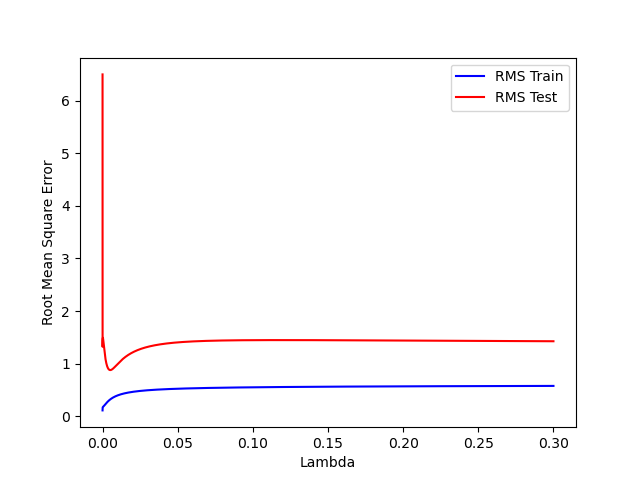
\includegraphics[scale=0.5]{img/Lambda_vs_RMS.png}
      \caption{Even with a slight increase in the regularization term $\lambda$, the RMS error on the testing set heavily decreases. }
      \label{fig:enter-label}
    \end{figure}

    \begin{theorem}[Least Squares Solution for Ridge Regression]
      The minimizer of the ridge loss is 
      \begin{equation}
        \hat{\beta} = (X^T X+ \lambda I)^{-1} X^T Y
      \end{equation}
    \end{theorem}
    \begin{proof}
      TBD
    \end{proof}

    \begin{theorem}[Bias Variance Decomposition of Ridge Regression]
      TBD 
    \end{theorem}

    From a computational point of view, we can see that by adding the $\lambda I$ term, it \textit{dampens} the matrix so that it does become invertible (or well conditioned), allowing us to find a solution. The higher the $\lambda$ term, the higher the damping effect. The next theorem compares the performance of the best ridge regression estimator to the best linear predictor. 

    \begin{theorem}[Hsu, Kakade, Zhang, 2014 \cite{hsu2014random}] 
      Suppose that $||X_i|| \leq r$ and let $\beta^T x$ be the best linear approximation to $m(x)$. Then, with probability at least $1 - 4 e^{-t}$, we have
      \begin{equation}
        r(\hat{\beta}) - r(\beta) \leq \bigg( 1 + O \bigg( \frac{1 + r^2 / \lambda}{n} \bigg) \bigg) \frac{\lambda ||\beta||^2}{2} + \frac{\sigma^2}{n} \frac{\Tr(\Sigma)}{2 \lambda}
      \end{equation}
    \end{theorem}

    We can see that the $\lambda$ term exists in the numerator on $\frac{\lambda ||\beta||^2}{2}$ and in the denominator on $\frac{\Tr(\Sigma)}{2 \lambda}$. This is the bias variance tradeoff. The first term is the bias term, which is the penalty for not being able to fit the data as well. The second term is the variance term, which is the penalty for having a more complex model. So our optimal $\lambda$ in the theoretical sense would be the one that minimizes the sum of these two terms. In practice, it's not this clean since we have unknown quantities in the formula, but just like how we did cross validation over the model complexity, we can also do cross validation over the $\lambda$. The decomposition above just gives you a theoretical feeling of how these things trade off. 

    \begin{code}[MWS of Ridge Regression in scikit-learn]
      \noindent\begin{minipage}{.6\textwidth}
      \begin{lstlisting}[]{Code}
        import numpy as np 
        from sklearn.linear_model import Ridge  

        X = np.random.randn(10, 5) 
        y = np.random.randn(10)
        # regularization parameter
        model = Ridge(alpha=1.0)  
        model.fit(X, y) 
        print(model.score(X, y))  
        print(model.intercept_)
        print(model.coef_) 
        print(model.predict(np.array([[1, 2, 3, 4, 5]]))) 
      \end{lstlisting}
      \end{minipage}
      \hfill
      \begin{minipage}{.39\textwidth}
      \begin{lstlisting}[]{Output}
        0.8605535024325397
        -0.28291076492665157
        [-0.10400521 -0.7587073  -0.05116735  1.16236649 -0.0401323 ]
        [2.39097184]
        .
        .
        .
        .
        .
        .
      \end{lstlisting}
      \end{minipage}
    \end{code}

    \begin{question}[To Do]
      Bayesian interpretation of ridge regression. 
    \end{question}

  \subsection{Forward Stepwise Regression} 

    Forward stepwise regression is a greedy algorithm that starts with an empty set of covariates and adds the covariate that most improves the fit. It avoids the NP-hardness of the best subset regression by adding covariates one by one. 

    \begin{definition}[Greedy Forward Stepwise Regression]
      Given your data $\mathcal{D}$, let's first standardize it to have mean $0$ and variance $1$.\footnote{This may or may not be a good idea, since the variance of each covariate can tell you a lot about the importance of the covariate.} You start off with a set $\mathcal{Q} = \{\}$ and choose the number of parameters $K$. 
      \begin{enumerate}
        \item With each covariate $X = (X_1, \ldots, X_n)$, we compute the correlation between it and the $Y$, which reduces to the inner product (since we standardized). 
        \begin{equation}
          \rho_j = \langle Y, X_{:, j} \rangle = \frac{1}{n} \sum_{i=1}^n Y_i X_{ji}
        \end{equation}

        \item Then, we take the covariate index that has the highest empirical correlation with $Y$, add it to $\mathcal{Q}$ and regress $Y$ only on this covariate. 
        \begin{equation}
          q_1 = \argmax_j \rho_j , \;\; \mathcal{Q} = \{q_1\}, \;\; \hat{\beta}_{q_1} = \argmin_{\beta} \frac{1}{n} ||Y - X_{:, q_1} \beta||^2 
        \end{equation}

        \item Then you repeat the process. You take the residual values $r = Y - X_{:, q_1} \hat{\beta}_{q_1} \in \mathbb{R}^n$ compute the correlation between $r$ and the remaining covariates, and pick our the maximum covariate index $q_2$. Then, you \textit{repeat the regression from start} with these two covariates 
        \begin{equation}
          q_2 = \argmax_j \langle r, X_{: ; j} \rangle , \;\; \mathcal{Q} = \{q_1, q_2\}, \;\; \hat{\beta}_{q_1, q_2} = \argmin_{\beta} \frac{1}{n} ||Y - X_{:,[q_1, q_2]} \beta||^2
        \end{equation}
        Note that you're not going to get the same coefficient for $\hat{\beta}_{q_1}$ as before since you're doing two variable regression. 

        \item You get out the residual values $r = Y - X_{:, [q_1, q_2]} \hat{\beta}_{q_1, q_2} \in \mathbb{R}^n$ and keep repeating this process until you have $K$ covariates in $\mathcal{Q}$. 
      \end{enumerate}
    \end{definition}

    Again, there is a bias variance tradeoff in choosing the number of covariates $K$, but through cross-validation, we can find the optimal $K$. It is also easy to add constraints, e.g. if we wanted to place a restriction that two adjacent covariates can't be chosen, we can easily add this to the algorithm. 

    \begin{theorem}[Rate of Convergence for Stepwise Regression]
      Let $\hat{f}_K$ be the optimal regressor we get from $K$ covariates in stepwise regression. Then, we have something like
      \begin{equation}
        ||f - \hat{f}||^2 \leq c ||f - f_K||^2 + \frac{\log{n}}{\sqrt{n}}
      \end{equation}
    \end{theorem}

    \subsubsection{Stagewise Regression} 

      Stagewise regression is a variant of forward stepwise regression where we add the covariate that most improves the fit, but we only take a small step in that direction. This is useful when we have a lot of covariates and we don't want to overfit. 

  \subsection{Lasso Regression}

    The Lasso approximates the best subset regression by using a convex relaxation. In particular, the norm $||\beta||_0$ is not convex, but the L1 norm $||\beta||_1$ is. Therefore, we want relax our constraint equation as such: 
    \begin{equation}
      \argmin_{||\beta||_0 \leq L} r(\beta) \mapsto \argmin_{||\beta||_1 \leq L} r(\beta)
    \end{equation}
    This gives us a convex problem, which we can then solve. In fact, it turns out that optimizing the risk given the L1 restriction on the norm is equivalent to minimizing the risk plus a L1 penalty, as this is the Lagrangian form of the original equation (this is in convex optimization). Therefore, there exists a pair $(L, \lambda)$ for which the two problems are equivalent 
    \begin{equation}
      \argmin_{||\beta||_1 \leq L} r(\beta) = \argmin_{\beta} r(\beta) + \lambda ||\beta||_1
    \end{equation}

    \begin{definition}[LASSO Regression]
      In \textbf{lasso regression}, we minimize the loss defined
      \begin{equation}
        \hat{R} (\beta) = \frac{1}{n} \sum_{i=1}^n (y^{(i)} - \beta^T x^{(i)})^2 + \lambda ||\beta||_1
      \end{equation}
      where we penalize according to the L1 norm of the coefficients. 
    \end{definition}
  
    A question arises: Why use the L1 norm? The motivation behind this is that we want to model the L0 norm as much as possible but at the same time we want it to be convex. This turns out to be precisely the L1 norm. Unfortunately, there is no closed form solution for this estimator, but in convex optimization, we can prove that this estimator is sparse. That is, for large enough $\lambda$, many of the components of $\hat{\beta}$ are $0$. The classical intuition for this is the figure below, where the equipotential lines have ``corners.'' In fact for any $0 < p < 1$, there are also corners, but the problem with using these p-norms is that they are not convex. 

    \begin{figure}[H]
      \centering 
      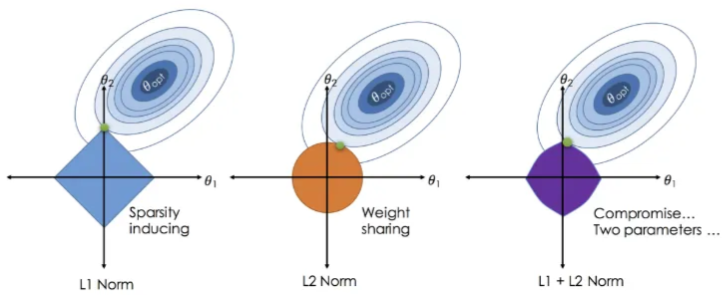
\includegraphics[scale=0.5]{img/regularizers.png}
      \caption{The ridge regularizer draws equipotential circles in our parameter space. The lasso draws a diamond, which tends to give a sparser solution since the loss is most likely to ``touch'' the corners of the contour plots of the regularizer. The elastic net is a linear combination of the ridge and lasso regularizers.} 
      \label{fig:regularizers_visual}
    \end{figure}

    To motivate this even further, let us take the two vectors 
    \begin{align}
      a = \bigg( \frac{1}{\sqrt{d}}, \ldots, \frac{1}{\sqrt{d}} \bigg) \qquad b = ( 1, 0, \ldots, 0)
    \end{align}
    Then the L0, L1, and L2 norms of $a$ are $d, \sqrt{d}, 1$ and those of $b$ are $1, 1, 1$. We want to choose a norm that capture the sparsity of $b$ and distinguishes it from $b$., The L0 norm clearly does this, but the L2 norm does not. The L1 norm is a good compromise between the two. 

    This now raises the question of how to determine a suitable regularization parameter $\lambda$. The next theorem shows a nice concentration property of the Lasso for bounded covariates. 

    \begin{theorem}[Concentration of Lasso]
      Given $(X, Y)$, assume that $|Y| \leq B$ and $\max_j |X_j| \leq B$. Let 
      \begin{equation}
        \beta^\ast = \argmin_{||\beta||_1 \leq L} r(\beta)
      \end{equation}
      be the best sparse linear predictor in the L1 sense, where $r(\beta) = \mathbb{E}[ (Y - \beta^T X)^2]$. Let our lasso estimator be 
      \begin{equation}
        \hat{\beta} = \argmin_{||\beta||_1 \leq L} \hat{r}(\beta) = \argmin_{||\beta||_1 \leq L} \frac{1}{n} \sum_{i=1}^n (Y_i - \beta^T X_i)^2
      \end{equation}
      which minimizes the empirical risk. Then, with probability at least $1 - \delta$, 
      \begin{equation}
        r(\hat{\beta}) \leq r(\beta^\ast) + \sqrt{\frac{16(L+1)^4 B^2}{n} \log \bigg( \frac{\sqrt{2} d}{\sqrt{\delta}} \bigg)} 
      \end{equation}
    \end{theorem}
    \begin{proof}
      
    \end{proof}

    \begin{code}[MWS of Lasso Regression in scikit-learn]
      \noindent\begin{minipage}{.6\textwidth}
      \begin{lstlisting}[]{Code}
        from sklearn.linear_model import Lasso

        X = np.random.randn(10, 5) 
        y = np.random.randn(10)
        # regularization parameter
        model = Lasso(alpha=1e-1)  
        model.fit(X, y) 
        print(model.score(X, y))  
        print(model.intercept_)
        print(model.coef_) 
        print(model.predict(np.array([[1, 2, 3, 4, 5]]))) 
      \end{lstlisting}
      \end{minipage}
      \hfill
      \begin{minipage}{.39\textwidth}
      \begin{lstlisting}[]{Output}
        0.47590269719236045
        -0.8861298412689853
        [0.         0.10767647 0.24172197 0.7427863  0.        ]
        [3.02553422]
        .
        .
        .
        .
        .
      \end{lstlisting}
      \end{minipage}
    \end{code}

    \subsubsection{Soft Thresholding and Proximal Gradient Descent} 

  \subsection{Bayesian Regularization with Priors}

    We will now demonstrate how having a normal $\alpha \mathbf{I}$ prior around the origin in a Bayesian setting is equivalent to having a ridge penalty of $\lambda = \sigma^2 / \alpha^2$ in a frequentist setting. If we have a Gaussian prior of form 
    \[p(\mathbf{w} \mid \alpha^2) = N(\mathbf{w} \mid \mathbf{0}, \alpha^2 \mathbf{I}) = \bigg( \frac{1}{2 \pi \alpha^2} \bigg)^{M/2} \exp \bigg( -\frac{1}{2\alpha^2} ||\mathbf{w}||^2_2 \bigg)\]
    We can use Bayes rule to compute 
    \begin{align*}
        p(\mathbf{w} \mid \mathbf{X}, \mathbf{Y}, \alpha^2, \sigma^2) & \propto p(\mathbf{Y} \mid \mathbf{w}, \mathbf{X}, \alpha^2, \sigma^2) \, p(\mathbf{w} \mid \mathbf{X}, \alpha^2, \sigma^2) \\
        & = \bigg[ \prod_{n=1}^N p(y^{(n)} \mid \mathbf{w}, \mathbf{x}^{(n)}, \alpha^2, \sigma^2 )\bigg] \, p(\mathbf{w} \mid \mathbf{X}, \alpha^2, \sigma^2) \\
        & = \bigg[ \prod_{n=1}^N \frac{1}{\sqrt{2 \pi \sigma^2}} \exp \bigg( - \frac{(y^{(n)} - h_\mathbf{w} (x^{(n)}))^2}{2 \sigma^2} \bigg) \bigg] \cdot \bigg( \frac{1}{2 \pi \alpha^2} \bigg)^{M/2} \exp \bigg( -\frac{1}{2\alpha^2} ||\mathbf{w}||^2_2 \bigg)
    \end{align*}
    and taking the negative logarithm gives us 
    \[\ell(\mathbf{w}) = \frac{1}{2\sigma^2} \sum_{n=1}^N \big(y^{(n)} - h_\mathbf{w} (\mathbf{x}^{(n)}) \big)^2 + \frac{N}{2}\ln{\sigma^2} + \frac{N}{2} \ln(2\pi) - \frac{M}{2} \ln(2\pi \alpha^2) + \frac{1}{2 \alpha^2} ||\mathbf{w}||_2^2\]
    taking out the constant terms relative to $\mathbf{w}$ and multiplying by $2 \sigma^2$ (which doesn't affect optima) gives us the ridge penalized error with a penalty term of $\lambda = \sigma^2 / \alpha^2$. 
    \[E(\mathbf{w}) = \frac{1}{2} \sum_{n=1}^N \big(y^{(n)} - h_\mathbf{w} (\mathbf{x}^{(n)}) \big)^2 + \frac{\sigma^2}{\alpha^2} ||\mathbf{w}||_2^2\]
    But minimizing this still gives a point estimate of $\mathbf{w}$, which is not the full Bayesian treatment. In a Bayesian setting, we are given the training data $(\mathbf{X}, \mathbf{Y})$ along with a new test point $\mathbf{x}^\prime$ and want to evaluate the predictive distribution $p(y \mid \mathbf{x}^\prime, \mathbf{X}, \mathbf{Y})$. We can do this by integrating over $\mathbf{w}$. 
    \begin{align*}
        p(y \mid \mathbf{x}^\prime, \mathbf{X}, \mathbf{Y}) & = \int p(y \mid \mathbf{x}^\prime, \mathbf{w}, \mathbf{X}, \mathbf{Y}) \, p(\mathbf{w} \mid \mathbf{x}^\prime, \mathbf{X}, \mathbf{Y}) \, d \mathbf{w} \\
        & = \int p(y \mid \mathbf{x}^\prime, \mathbf{w}) \, p(\mathbf{w} \mid \mathbf{X}, \mathbf{Y}) \, d \mathbf{w} 
    \end{align*}
    where we have omitted the irrelevant variables, along with $\alpha^2$ and $\sigma^2$ to simplify notation. By substituting the posterior $p(\mathbf{w} \mid \mathbf{X}, \mathbf{Y})$ with a normalized version of our calculation above and by noting that 
    \[p(y \mid \mathbf{x}^\prime, \mathbf{w}) = N(y \mid h_\mathbf{w} (\mathbf{x}^\prime), \sigma^2) = \frac{1}{\sqrt{2 \pi \sigma^2}} \exp \bigg( -\frac{\big(y - h_\mathbf{w} (\mathbf{x}^\prime)\big)^2}{2 \sigma^2} \bigg)\]
    Now this integral may or may not have a closed form, but if we consider the polynomial regression with the hypothesis function of form 
    \[h_\mathbf{w} (x) = w_0 + w_1 x + w_2 x^2 + \ldots + w_{M-1} x^{M-1}\]
    then this integral turns out to have a closed form solution given by 
    \[p(y \mid \mathbf{x}^\prime, \mathbf{X}, \mathbf{Y}) = N \big( y \mid m(x^\prime), s^2 (x^\prime)\big)\]
    where 
    \begin{align*}
        m(x^\prime) & = \frac{1}{\sigma^2} \boldsymbol{\phi}(x^\prime)^T \mathbf{S} \bigg( \sum_{n=1}^N \boldsymbol{\phi}(x^{(n)}) y^{(n)} \bigg) \\
        s^2 (x^\prime) & = \sigma^2 + \boldsymbol{\phi}(x^\prime)^T \mathbf{S} \boldsymbol{\phi}(x^\prime) \\
        \mathbf{S}^{-1} & = \alpha^{-2} \mathbf{I} + \frac{1}{\sigma^2} \sum_{n=1}^N \boldsymbol{\phi}(x^{(n)}) \boldsymbol{\phi}(x^\prime)^T 
    \end{align*}
    and $\boldsymbol{\phi}(x)$ is the vector of functions $\phi_i (x) = x^i$ from $i = 0, \ldots, M-1$. 



\section{Logistic and Softmax Regression} 

  We can upgrade from a discriminant function to a discriminative probabilistic model with \textbf{logistic regression}. In practice, we usually deal with \textbf{probabilistic models} where rather than giving a point estimate $\hat{y}$, we attempt to model the \textit{distribution} $\mathbb{P}_{Y \mid X = \hat{x}}$. Even though in the end, we will just output the mean $\mu$ of this conditional distribution, modeling the distribution allows us to quantify uncertainty in our measurements. 

  \begin{definition}[Logistic Regression]
    The \textbf{logistic regression} model is a linear model of the form 
    \begin{equation}
      f_w (x) = \sigma (w^T x) = \frac{1}{1 + e^{- w^T x}}, \text{ where } \sigma(x) \coloneqq \frac{1}{1 + e^{x}}
    \end{equation}
    It is different from linear regression in two ways: 
    \begin{enumerate}
      \item In linear regression, we assumed that the targets are linearly dependent with the covariates as $y = w^T x + b$. However, this means that the hypothesis $f_w$ is unbounded. Since we have two classes (say with labels $0$ and $1$), we must have some sort of \textit{link function} $\sigma$ that takes the real numbers and compresses it into the domain $[0, 1]$. Technically, we can choose any continuous, monotinically increasing function from $\mathbb{R}$ to $(0, 1)$. However, the following property of the sigmoid makes derivation of gradients very nice. 
        \begin{equation}
          \sigma^\prime (x) = \sigma(x) \, \big(1 - \sigma(x) \big)
        \end{equation}
      \item Once this is compressed, we assume that the residual distribution is a Bernoulli. 
    \end{enumerate}
  \end{definition}

  \begin{definition}[Binary Cross Entropy Loss as Surrogate Loss for Logistic Regression]
    The surrogate loss for logistic regression is the \textbf{binary cross entropy loss}, which is defined as
    \begin{equation}
      L(y, \hat{y}) = -y \log \hat{y} - (1 - y) \log (1 - \hat{y})
    \end{equation}
  \end{definition}

  One important observation to make is that notice that the output of our hypothesis is used as a parameter to define our residual distribution. 
  \begin{enumerate}
    \item In linear regression, the $f_w$ was used as the \textit{mean} $\mu$ of a Gaussian. 
    \item In logistic regression, the $f_w$ is used also as the mean $p$ of a Bernoulli. 
  \end{enumerate}
  The reason we want this sigmoid is so that we make the domains of the means of the residuals match the range of the outputs of our model. It's simply a manner of convenience, and in fact we could have really chose any function that maps $\mathbb{R}$ to $(0, 1)$. 

  Some questions may arise, such as ``why isn't the variance parameter of the Gaussian considered in the linear model?" or ``what about other residual distributions that have multiple parameters?" This is all answered by generalized linear models, which uses the output of a linear model as a \textit{natural parameter} of the canonical exponential family of residual distributions. 

  Unfortunately, there is no closed form solution for logistic regression like the least squares solution in linear regression. Therefore, we can only resort to maximum likelihood estimation. 

  \begin{theorem}[Maximum Likelihood Estimation for Logistic]
    Given a dataset $\mathcal{D} = \{(x^{(i)}, y^{(i)})\}_{i=1}^N$, our likelihood is 
    \begin{equation}
      L(\theta ; \mathcal{D}) = \prod_{i=1}^n p(y^{(i)} \;|\; x^{(i)} ; \theta) = \prod_{i=1}^N  \big( h_\theta (x^{(i)} )\big)^{y^{(i)}} \; \big( 1 - h_\theta (x^{(i)})\big)^{1-y^{(i)}}
    \end{equation}
    We can equivalently minimize its negative log likelihood, giving us the \textbf{binary cross entropy} loss function
    \begin{align}
      \ell(\theta) & = -\log L(\theta) \\
      & = -\sum_{i=1}^n y^{(i)} \log h_\theta (x^{(i)}) + (1 - y^{(i)}) \log (1 - h_\theta (x^{(i)}))
    \end{align}
    Now taking the gradient for just a single sample $(x^{(i)}, y^{(i)})$ gives 
    \begin{align}
        \frac{\partial \ell}{\partial \theta}  & = \bigg( \frac{y^{(i)}}{\sigma(\theta^T x^{(i)})} - \frac{1 - y^{(i)}}{1 - \sigma(\theta^T x^{(i)})} \bigg) \, \frac{\partial}{\partial \theta} \sigma (\theta^T x^{(i)}) \\
        & = \frac{\sigma(\theta^T x^{(i)}) - y^{(i)}}{\sigma(\theta^T x^{(i)}) \, \big( 1 - \sigma(\theta^T x^{(i)}) \big)} \sigma(\theta^T x^{(i)}) \, \big( 1 - \sigma(\theta^T x^{(i)}) \big) x^{(i)} \\
        & = \big( h_\theta (x^{(i)}) - y^{(i)} \big) x
    \end{align}
    and summing it over some minibatch $M \subset \mathcal{D}$ gives 
    \begin{equation}
      \nabla_\theta \ell_M = \sum_{(x, y) \in M} (y - h_\theta(x)) x
    \end{equation}
    Therefore, the stochastic gradient descent algorithm is 
    \begin{align}
      \theta & = \theta - \eta \nabla_\theta \ell (\theta) \\
      & = \theta - \eta \sum_{(x, y) \in M} (y - h_\theta(x)) x
    \end{align}
  \end{theorem}

  We would like to extend this to the multiclass case. 

  \begin{definition}[Softmax Function]
    The softmax function is defined 
    \begin{equation}
      o(\mathbf{x}) = \frac{e^{\mathbf{x}}}{||e^{\mathbf{x}}||} = \frac{1}{\sum_j e^{x_j}}\begin{pmatrix} e^{x_1} \\ \vdots \\ e^{x_D} \end{pmatrix}
    \end{equation}
  \end{definition}

  What makes the softmax so popular is that the total derivative turns out to simplify functions a lot. The total derivative of the softmax can be derived as such. 

  \begin{lemma}[Derivative of Softmax]
    The derivative of the softmax is 
    \begin{equation}
      D o (\mathbf{x}) = \mathrm{diag}(o (\mathbf{x})) - o (\mathbf{x}) \otimes o (\mathbf{x})
    \end{equation}
    where $\otimes$ is the outer product. That is, let $y_i$ be the output of the softmax. Then, for the $4 \times 4$ softmax function, we have 
    \begin{equation}
      D o(\mathbf{x}) = \begin{pmatrix} y_1 (1 - y_1) & - y_1 y_2 & -y_1 y_3 & - y_1 y_4 \\ -y_2 y_1 & y_2 (1 - y_2) & - y_2 y_3 & - y_2 y_4 \\ -y_3 y_1 & y_3 y_3 & y_3 (1 - y_3) & -y_3 y_4 \\ -y_4 y_1 & -y_4 y_2 & -y_4 y_3 & y_4 (1 - y_4) \end{pmatrix}
    \end{equation}
  \end{lemma}
  \begin{proof}
    We will provide a way that allows us not to use quotient rule. Given that we are taking the partial derivative of $y_i$ with respect to $x_j$, we can use the log of it to get 
    \[\frac{\partial}{\partial x_j} \log (y_i) = \frac{1}{y_i} \frac{\partial y_i}{\partial x_j} \implies \frac{\partial y_i}{\partial x_j} = y_i \, \frac{\partial}{\partial x_j} \log(y_i)\]
    Now the partial of the log term is 
    \begin{align}
      \log{y_i} & = \log \bigg( \frac{e^{x_i}}{\sum_l e^{x_l}} = x_i - \log \bigg( \sum_l e^{x_l}\bigg) \\
      \frac{\partial}{\partial x_j} \log(y_i) & = \frac{\partial x_i}{\partial x_j} - \frac{\partial}{\partial x_j} \log \bigg( \sum_l e^{x_l}\bigg) \\
      & = 1_{i = j} - \frac{1}{\sum_l e^{x_l}} e^{x_j}
    \end{align}
    and plugging this back in gives 
    \begin{equation}
      \frac{\partial y_i}{\partial x_j} = y_i (1_{i = j} - y_j)
    \end{equation}
  \end{proof}

  It also turns out that the sigmoid is a specific case of the softmax. That is, given softmax for 2 classes, we have 
  \begin{equation}
    o\begin{pmatrix} x_1 \\ x_2 \end{pmatrix} = \frac{1}{e^{x_1} + e^{x_2}} \begin{pmatrix} e^{x_1} \\ e^{x_2} \end{pmatrix}
  \end{equation}
  So, the probability of being in class $1$ is 
  \begin{equation}
    \frac{e^{x_1}}{e^{x_1} + e^{x_2}} = \frac{1}{1 + e^{x_2 - x_1}}
  \end{equation}
  and the logistic sigmoid is just a special case of the softmax function that avoids using redundant parameters. We actually end up overparameterizing the softmax because the probabilities must add up to one. 

  \begin{definition}[Softmax Regression Model]
    The softmax regression of $K$ classes assumes a model of the form 
    \begin{equation}
      h_\theta (x) = o ( \mathbf{W} \mathbf{x} + \mathbf{b})
    \end{equation}
    where $\mathbf{W} \in \mathbb{R}^{K \times D}, \mathbf{b} \in \mathbb{R}^D$. Again, we have a linear map followed by some link function (the softmax) which allows us to nonlinearly map our unbounded linear outputs to some domain that can be easily parameterized by a probability distribution. In this case, our residual distribution is a \textbf{multinomial distribution} 
    \begin{equation}
      y \sim \mathrm{Multinomial}\big( h_\mathbf{w} (\mathbf{x}) \big) = \mathrm{Multinomial}\big( [h_\mathbf{w} (\mathbf{x})]_1, \ldots, [h_\mathbf{w} (\mathbf{x})]_K \big)
    \end{equation}
  \end{definition}

  \begin{definition}[Multiclass Cross Entropy Loss as Surrogate Loss for Softmax]
    The surrogate loss for softmax regression is the \textbf{multiclass cross entropy loss}, which is defined as 
    \begin{equation}
      L(\theta ; \mathcal{D}) = - \sum_{i=1}^N \sum_{k=1}^K y_k^{(i)} \log \big( h_\theta (\mathbf{x}^{(i)}) \big)_k
    \end{equation}
  \end{definition}

  \begin{theorem}[Maximum Likelihood Estimation for Softmax]
    Since a closed form solution is not available for logistic regression, it is clearly not available for softmax. Therefore, we one hot encode our target variables as $\mathbf{y}^{(i)}$ and write our likelihood as 
    \begin{equation}
      L(\theta; \mathcal{D}) = \prod_{i=1}^N \prod_{k=1}^K p(C_k \mid \mathbf{x}^{(i)})^{\mathbf{y}^{(i)}_k} = \prod_{i=1}^N \prod_{k=1}^K \big( \mathbf{h}_\mathbf{W} (\mathbf{x}^{(i)})\big)_k^{\mathbf{y}_k^{(i)}}
    \end{equation}
    Taking the negative logarithm gives us the \textbf{cross entropy} loss function
    \begin{equation}
      \ell (\boldsymbol{\theta}) = - \sum_{i=1}^N \sum_{k=1}^K y^{(i)}_k \log \big( \mathbf{h}_{\boldsymbol{\theta}} (\mathbf{x}^{(i)})\big)_k = - \sum_{i=1}^N \mathbf{y}^{(i)} \dot \log \big( \mathbf{h}_{\boldsymbol{\theta}} (\mathbf{x}^{(i)} \big)
    \end{equation}
    where $\cdot$ is the dot product. The gradient of this function may seem daunting, but it turns out to be very cute. Let us take a single sample $(\mathbf{x}^{(i)}, \mathbf{y}^{(i)})$, drop the index $i$, and write
    \begin{align*}
      \mathbf{x} & \mapsto \mathbf{W} \mathbf{x} + \mathbf{b} = \mathbf{z} \\
      \hat{\mathbf{y}} = \mathbf{a} & = o (\mathbf{z}) \\
      L & = - \mathbf{y} \cdot \log (\mathbf{a}) = - \sum_{k=1}^K y_k \log(a_k)
    \end{align*}
    We must compute 
    \begin{equation}
      \frac{\partial L}{\partial \mathbf{W}} = \frac{\partial L}{\partial \mathbf{a}} \frac{\partial \mathbf{a}}{\partial \mathbf{z}} \frac{\partial \mathbf{z}}{\partial \boldsymbol{\theta}}
    \end{equation}
    We can compute $\partial L /\partial \mathbf{z}$ as such, using our derivations for the softmax derivative above. We compute element wise. 
    \begin{align*}
      \frac{\partial L}{\partial z_j} & = - \sum_{k=1}^K y_k \, \frac{\partial}{\partial z_j} \log (a_k) \\
      & = - \sum_{k=1}^K y_k \frac{1}{a_k} \frac{\partial a_k}{\partial z_j} \\
      & = - \sum_{k=1}^K \frac{y_k}{a_k} \, a_k (1_{\{k = j\}} - a_j) \\
      & = - \sum_{k=1}^K y_k (1_{\{k = j\}} - a_j) \\
      & = \bigg( \sum_{k=1}^K y_k a_j \bigg) - y_j \\
      & = a_j \bigg( \sum_{k=1}^K y_k \bigg) - y_j \\
      & = a_j - y_j
    \end{align*}
    and combining these gives 
    \begin{equation}
      \frac{\partial L}{\partial \mathbf{z}} = (\mathbf{a} - \mathbf{y})^T
    \end{equation}
    Now, computing $\partial \mathbf{z} / \partial \mathbf{W}$ gives us a $3$-tensor, which is not ideal to work with. However, let us just compute this with respect to the elements again. We have 
    \begin{align*}
      z_k & = \sum_{d=1}^D W_{kd} x_d + b_k \\ 
      \frac{\partial z_k}{\partial W_{ij}} & = \sum_{d=1}^D x_d \frac{\partial}{\partial W_{ij}} W_{kd}
    \end{align*}
    where 
    \begin{equation}
      \frac{\partial}{\partial W_{ij}} W_{kd} = \begin{cases} 1 & \text{ if } i = k, j = d \\ 0 & \text{ else} \end{cases}
    \end{equation}
    Therefore, since $d$ is iterating through all elements, the sum will only be nonzero if $k = i$. That is, $\frac{\partial z_k}{\partial W_{ij}} = x_j$ if $k = i$ and $0$ if else. Therefore, 
    \begin{center}
      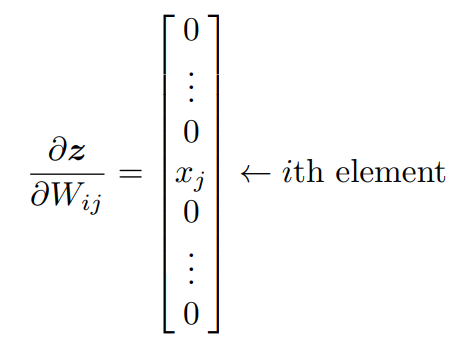
\includegraphics[scale=0.3]{img/softmax_deriv.png}
    \end{center}
    Now computing 
    \begin{equation}
      \frac{\partial L}{\partial W_{ij}} = \frac{\partial L}{\partial \mathbf{z}} \frac{\partial \mathbf{z}}{\partial W_{ij}} = (\mathbf{a} - \mathbf{y}) \frac{\partial \mathbf{z}}{\partial W_{ij}} = \sum_{k=1}^K (a_k - y_k) \frac{\partial z_k}{\partial W_{ij}} = (a_i - y_i) x_j
    \end{equation}
    To get $\partial L / \partial W_{ij}$ we want a matrix whose entry $(i, j)$ is $(a_i - y_i) x_j$. This is simply the outer product as shown below. For the bias term, $\partial \mathbf{z} / \partial \mathbf{b}$ is simply the identity matrix. 
    \begin{equation}
      \frac{\partial L}{\partial \mathbf{W}} = (\mathbf{a} - \mathbf{y}) \mathbf{x}^T, \;\;\;\; \frac{\partial L}{\partial \mathbf{b}} = \mathbf{a} - \mathbf{y}
    \end{equation}

    Therefore, summing the gradient over some minibatch $M \subset [N]$ gives 
    \begin{equation}
      \nabla_{\mathbf{W}} \ell_M = \sum_{i \in M} (\mathbf{h}_{\boldsymbol{\theta}}(\mathbf{x}^{(i)}) - \mathbf{y}^{(i)}) (\mathbf{x}^{(i)})^T, \;\;\;\;\; \nabla_{\mathbf{b}} \ell_M = \sum_{i \in M} (\mathbf{h}_{\boldsymbol{\theta}}(\mathbf{x}^{(i)}) - \mathbf{y}^{(i)})
    \end{equation}
    and our stochastic gradient descent algorithm is 
    \begin{align*}
      \boldsymbol{\theta} = \begin{pmatrix} \mathbf{W} \\ \mathbf{b} \end{pmatrix} & = \begin{pmatrix} \mathbf{W} \\ \mathbf{b} \end{pmatrix} - \eta \begin{pmatrix} \nabla_{\mathbf{W}} \ell_M \\ \nabla_{\mathbf{b}} \ell_M \end{pmatrix} \\
      & = \begin{pmatrix} \mathbf{W} \\ \mathbf{b} \end{pmatrix} - \eta \begin{pmatrix} \sum_{i \in M} (\mathbf{h}_{\boldsymbol{\theta}}(\mathbf{x}^{(i)}) - \mathbf{y}^{(i)}) (\mathbf{x}^{(i)})^T \\ \sum_{i \in M} (\mathbf{h}_{\boldsymbol{\theta}}(\mathbf{x}^{(i)}) - \mathbf{y}^{(i)}) \end{pmatrix} 
    \end{align*}
  \end{theorem}

\section{Generalized Linear Models} 

  Remember the linear model looked like this, where we use the conventional $\beta$ notation to represent parameters. 
  \begin{equation}
    Y = X^T \beta + \epsilon, \;\; \epsilon \sim N(0, \sigma^2 I)
  \end{equation}
  which implies that $Y \mid X \sim N(X^T \beta, \sigma^2 I)$. Basically, given $x$, I assume some distribution of $Y$, and the value of $x$ will help me guess what the mean of this distribution is. Note that we in here assume that only the mean depends on $X$. I could potentially have something crazy, like 
  \[Y \mid X \sim N(X^T \beta, (X^T \gamma) (X X^T + I))\]
  where the covariance will depend on $X$, too, but in this case we only assume that that mean is dependent on $X$. 
  \[Y \mid X \sim N(\mu(X), \sigma^2 I)\]
  where in the linear model, $\mu(X) = X^T \beta$. So, there are three assumptions we are making here: 
  \begin{enumerate}
    \item $Y \mid X$ is Gaussian. 
    \item $X$ only affects the mean of $Y \mid X$, written $\mathbb{E}[Y \mid X] = \mu(X)$. 
    \item $X$ affects the mean in a linear way, such that $\mu(X) = X^T \beta$. 
  \end{enumerate}
  So the two things we are trying to relax are: 
  \begin{enumerate}
    \item \textbf{Random Component}: the response variable $Y \mid X$ is continuous and normally distributed with mean $\mu = \mu(X) = \mathbb{E}[Y \mid X]$. 
    \item \textbf{Link}: I have a link that explains the relationship between the $X$ and the $\mu$, and this relationship is $\mu(X) = X^T \beta$. 
  \end{enumerate}
  So when talking about GLMs, we are not changing the fact that we have a linear function $X \mapsto X^T \beta$. However, we are going to assume that $Y \mid X$ now comes from a broader \textbf{family of exponential distributions}. Second, we are going to assume that there exists some \textbf{link function} $g$
  \[g(\mu(X)) = X^T \beta\]
  Admittedly, this is not the most intuitive way to think about it, since we would like to have $\mu(X) = f(X^T \beta)$, but here we just decide to call $f = g^{-1}$. Therefore, if I want to give you a GLM, I just need to give you two things: the conditional distribution $Y \mid X$, which can be any distribution in the exponential family, and the link function $g$. 

  We really only need this link function due to compatibility reasons. Say that $Y \mid X \sim \mathrm{Bern}(p)$. Then, $\mu(X) = \mathbb{E}[Y \mid X]$ always lives in $[0, 1]$, but $X^T \beta$ always lives in $\mathbb{R}$. We want our model to be realistic, and we can clearly see the problem shown in Figure \ref{fig:Bernoulli_GLM}. 

  \begin{figure}[H]
    \centering
    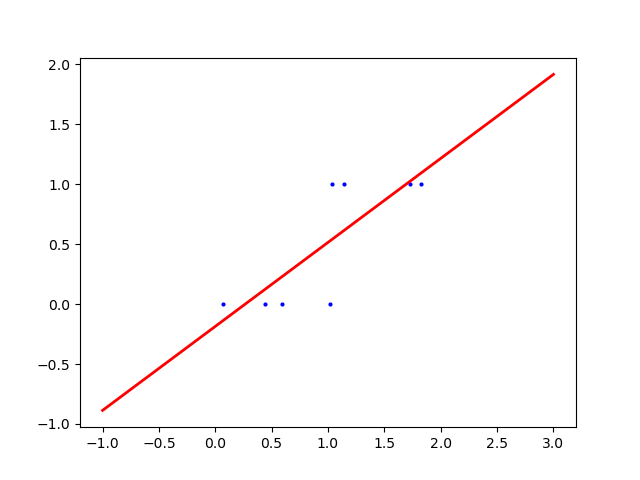
\includegraphics[scale=0.5]{img/GLM_bernoulli.png}
    \caption{Fitting a linear model for Bernoulli random variables will predict a mean that is outside of $[0, 1]$ when getting new datapoints. }
    \label{fig:Bernoulli_GLM}
  \end{figure}

  If $Y \mid X$ is some exponential distribution, then its support is always positive and so $\mu(X) > 0$. But if we stick to the old form of $\mu(X) = X^T \beta$, then $\mathrm{Im}(\mu) = \mathbb{R}$, which is not realistic when we predict negative values. Let's take a couple examples: 

  \begin{example}[Disease Epidemic]
    In the early stages of a disease epidemic, the rate at which new cases occur can often increase exponentially through time. Clearly, $\mu(X) = \mathbb{E}[Y \mid X]$ should be positive and we should have some sort of exponential trend. Hence, if $\mu(x)$ is the expected number of cases on data $x$, a model of the form 
    \begin{equation}
      \mu(x) = \gamma \exp (\delta x)
    \end{equation}
    seems appropriate, where $\gamma$ and $\delta$ are simply scaling factors. Clearly, $\mu(X)$ is not of the form $f(X^T \beta)$. So what I do is to transform $\mu$ in such a way that I can get something that is linear. 
    \begin{equation}
      \log(\mu(X)) = \log(\gamma) + \delta X
    \end{equation}
    which is now linear in $X$, of form $\beta_0 + \beta_1 X$. This will have some effects, but this is what needs to be done to have a genearlized linear model. Note that what I did to $\mu$ was take the log of it, and so the link function is $g = \log$, called the \textbf{log-link}. Now that we have chosen the $g$, we still need to choose what the conditional distribution $Y \mid X$ would be. This is determined by speaking with industry professionals, experience, and convenience. In this case, $Y$ is a count, and since this must be a discrete distribution. Since it is not bounded above, we think Poisson. 
  \end{example}

  \begin{example}[Prey Capture Rate]
    The rate of capture of preys, $Y$, by a hunting animal, tends to increase with increasing density of prey $X$, but eventually level off when the predator is catching as much as it can cope with. We want to find a perhaps concave function that levels off, and suitable model might be 
    \begin{equation}
      \mu(X) = \frac{\alpha X}{h + X}
    \end{equation}
    where $\alpha$ represents the maximum capture rate, and $h$ represents the prey density at which the capture rate is half the maximum rate. Again, we must find some transformation $g$ that turns this into a linear function of $X$, and what we can do it use the \textbf{reciprocal-link}. 
    \begin{equation}
      \frac{1}{\mu(X)} = \frac{h + X}{\alpha X} = \frac{h}{\alpha} \frac{1}{X} + \frac{1}{\alpha}
    \end{equation}
    The standard deviation of capture rate might be approximately proportional to the mean rate, suggesting the use of a Gamma distribution for the response. 
  \end{example}

  \begin{example}[Kyphosis Data]
    The Kyphosis data consist of measurements on $81$ children following corrective spinal surgery. The binary response variable, Kyphosis, indicates the presence or absence of a postoperative deforming. The three covariates are: age of the child in months, number of the vertebrae involved in the operation, and the start of the range of the vertebrae involved. The response variable is binary so there is no choice: $Y \mid X$ is Bernoulli with expected value $\mu(X) \in (0, 1)$. We cannot write $\mu(X) = X^T \beta$ because the right hand side ranges through $\mathbb{R}$, and so we find an invertible function that squishes $\mathbb{R}$ to $(0, 1)$, and so we can choose basically any CDF. 
  \end{example}

  For clarification, when writing a distribution like $\mathrm{Bernoulli}(p)$, or $\mathrm{Binomial}(n, p)$, $\mathrm{Poisson}(\lambda)$, or $N(\mu, \sigma^2)$, the hyperparameters that we usually work with we will denote as $\boldsymbol{\theta}$, and the space that this $\boldsymbol{\theta}$ lives in will denote $\Theta$. For example, for the Bernoulli, $\Theta = [0, 1]$, and for Poisson, $\Theta = [0, +\infty)$. 

  Ultimately, a GLM consists of three steps: 
  \begin{enumerate}
    \item The observed input $X$ enters the model through a linear function $\beta^T X$. 
    \item The conditional mean of response, is represented as a function of the linear combination 
      \begin{equation}
        \mathbb{E}[Y \mid X] = \mu = f(\beta^T X)
      \end{equation}
    \item The observed response is drawn from an exponential family distribution with conditional mean $\mu$. 
  \end{enumerate}

  \subsection{Exponential Family}

    We can write the pdf of a distribution as a function of the input $x$ and the hyperparameters $\theta$, so we can write $P_\theta (x) = p(\theta, x)$. For now, let's think that both $x, \theta \in \mathbb{R}$. Think of all the functions that depend on $\theta$ and $x$. There are many of them, but we want $\theta$ and $x$ to interact in a certain way. The way that I want them to interact with each other is that they are multiplied within an exponential term. Now clearly, this is not a very rich family, so we are just slapping some terms that depend only on $\theta$ and only on $x$. 
    \[p_\theta (x) = \exp(\theta x) h(x) c(\theta)\]
    But now if $\theta \in \mathbb{R}^k$ and $x \in \mathbb{R}^q$, then we cannot simply take the product nor the inner product, but what we can do is map both of them into a space that has the same dimensions, so I can take the inner product. That is, let us map $\boldsymbol{\theta} \mapsto \boldsymbol{\eta}(\boldsymbol{\theta}) \in \mathbb{R}^k$ and $\mathbf{x} \mapsto \mathbf{T}(\mathbf{x}) \in \mathbb{R}^k$, and so 
    our exponential distribution form would be generalized into something like 
    \[p_{\boldsymbol{\theta}} (\mathbf{x}) = \exp\big[ \boldsymbol{\eta}(\boldsymbol{\theta}) \cdot \mathbf{T}(\mathbf{x}) \big] h(\mathbf{x}) c(\boldsymbol{\theta})\]
    We can think of $c(\boldsymbol{\theta})$ as the normalizing term that allows us to integrate the pdf to $1$. 
    \[\int_\mathcal{X} p_{\boldsymbol{\theta}} (\mathbf{x}) = c(\boldsymbol{\theta}) \int \exp\big[\boldsymbol{\eta}(\boldsymbol{\theta}) \cdot \mathbf{T}(\mathbf{x}) \big] h(\mathbf{x})  \,d\mathbf{x}\]
    We can just push the $c(\boldsymbol{\theta})$ term into the exponential by letting $c(\boldsymbol{\theta}) = e^{-\log(c(\boldsymbol{\theta}))^{-1}}$ to get our definition. 

    \begin{definition}[Exponential Family]
      A \textbf{k-parameter exponential family} is a family of distributions with pdf/pmf of the form 
      \[p_{\boldsymbol{\theta}} (\mathbf{x}) = \exp\big[ \boldsymbol{\eta}(\boldsymbol{\theta}) \cdot \mathbf{T}(\mathbf{x}) - B(\boldsymbol{\theta}) \big] h(\mathbf{x})\]
      The $h$ term, as we will see, will not matter in our maximum likelihood estimation, so we keep it outside the exponential. 
      \begin{enumerate}
        \item $\boldsymbol{\eta}$ is called the \textbf{canonical parameter}. Given a distribution parameterized by the regular hyperparameters $\boldsymbol{\theta}$, we would like to parameterize it in a different way $\boldsymbol{\eta}$ under the function $\boldsymbol{\eta}: \Theta \rightarrow \mathbb{R}$
        \item $\mathbf{T}(\mathbf{x})$ is called the \textbf{sufficient statistic}. 
        \item $h(\mathbf{x})$ is a nonnegative scalar function. 
        \item $B(\boldsymbol{\theta})$ is the normalizing factor. 
      \end{enumerate}
    \end{definition}

    Let's look at some examples. 

    \begin{example}[Gaussian]
      If we put the coefficient into the exponential and expand the square term, we get 
      \[p_\theta (x) = \exp \bigg( \frac{\mu}{\sigma^2} \cdot x - \frac{1}{2\sigma^2} \cdot x^2 - \frac{\mu^2}{2 \sigma^2} - \log ( \sigma \sqrt{2 \pi}) \bigg)\] 
      where 
      \[\boldsymbol{\eta}(\boldsymbol{\theta}) = \begin{pmatrix} \mu /\sigma^2 \\ -1 / 2 \sigma^2 \end{pmatrix}, \; T(x) = \begin{pmatrix} x \\ x^2 \end{pmatrix}, \; B(\theta) = \frac{\mu^2}{2 \sigma^2} + \log(\sigma \sqrt{2 \pi}), \; h(x) = 1\]
      This is not a unique representation since we can take the $\log(\sqrt{2 \pi})$ out of the exponential, but why bother to do this when we can just stuff everything into $B$ and keep $h$ simple. 
    \end{example}

    \begin{example}[Gaussian with Known Variance]
      If we have known variance, we can write the Gaussian pdf as 
      \[p_\theta (x) = \exp \bigg[ \frac{\mu}{\sigma} \cdot \frac{x}{\sigma} - \frac{\mu^2}{2 \sigma^2} \bigg] \cdot \frac{1}{\sigma \sqrt{2\pi}} e^{x^2/2 \sigma^2}\]
      where 
      \[\eta(\theta) = \frac{\mu}{\sigma}, \; T(x) = \frac{x}{\sigma}, \; B(\theta) = \frac{\mu^2}{2 \sigma^2}, \; h(x) = \frac{1}{\sigma \sqrt{2 \pi}} e^{x^2/2 \sigma^2}\]
    \end{example}

    \begin{example}[Bernoulli]
    The pmf of a Bernoulli with $\theta$ is 
    \begin{align*}
        p_\theta (x) & = \theta^x (1 - \theta)^{(1 - x)} \\
        & = \exp \big[x \log (\theta) + (1 - x)\log(1 - \theta) \big] \\
        & = \exp \bigg( x \log \Big[ \frac{\theta}{1 - \theta} \Big] - \log \Big[ \frac{1}{1 - \theta} \Big] \bigg)
    \end{align*}
    where 
    \[\eta(\theta) = \log \Big[ \frac{\theta}{1 - \theta} \Big], \; T(x) = x, \; B(\theta) = \log \Big[ \frac{1}{1 - \theta} \Big], \; h(x) = 1\]
    \end{example}


    \begin{example}[Binomial with Known Number of Trials]
    We can transform a binomial with known $N$ as 
    \begin{align*}
      p_\theta (x) &  = \binom{N}{x} \theta^x  (1 - \theta)^{1 - x} \\
                   & = \exp \bigg[ x \ln \big( \frac{\theta}{1 - \theta} \Big) + \ln(1 - \theta) \bigg] \cdot \binom{N}{x} 
    \end{align*}
    where 
      \[\eta (\theta) = \ln \big( \frac{\theta}{1 - \theta} \Big), \; T(x) = x, \; B(\theta) = \ln(1 - \theta), \; h(x) = \binom{N}{x}\]
    \end{example}

    \begin{example}[Poisson]
    The pmf of Poisson with $\theta$ can be expanded 
    \begin{align*}
        p_\theta & = \frac{\theta^{-x}}{x!} e^{-\theta} \\
        & = \exp \big[ -\theta + x\log(\theta) - \log(x!) \big] \\
        & = \exp \big[ x \log(\theta) - \theta \big] \, \frac{1}{x!}
    \end{align*}
    where 
    \[\eta(\theta) = \log(\theta), \; T(x) = x, \; B(\theta) = \theta, \; h(x) = \frac{1}{x!}\]
    \end{example}

    However, the uniform is not in here. In fact, any distribution that has a support that does not depend on the parameter is not an exponential distribution. 

    Let us now focus on one parameter families where $\theta \in \Theta \subset \mathbb{R}$, which do not include the Gaussian (with unknown mean and variance, Gamma, multinomial, etc.), which has a pdf written in the form 
    \[p_\theta (x) = \exp \big[ \eta (\theta) \, T(x) - B(\theta) \big] \, h(x)\]


    \subsubsection{Canonical Exponential Family}

      Now a common strategy in statistical analysis is to reparamaterize a probability distribution. Suppose a family of probability distributions $\{P_\theta\}$ is parameterized by $\theta \in \Theta \subset \mathbb{R}$. If we have an invertible function $\eta: \Theta \rightarrow \mathcal{T} \subset \mathbb{R}$, then we can paramaterize the same family with $\eta$ rather than $\theta$, with no loss of information. Typically, it is the case that $\eta$ is invertible for exponential families, so we can just reparameterize the whole pdf and write 
      \[p_\eta (x) = \exp \big[ \eta \, T(x) - \phi(\eta) \big] \, h(x)\]
      where $\phi = B \circ \eta^{-1}$. 

      \begin{definition}[Canonical One-Parameter Exponential Family]
      A family of distributions is said to be in \textbf{canonical one-parameter exponential family} if its density is of form 
      \[p_\eta (x) = \exp \big[ \eta \, T(x) - \phi(\eta) \big] \, h(x)\]
      which is a subfamily of the exponential family. The function $\psi$ is called the \textbf{cumulant generating function}. 
      \end{definition}

      Before we move on, let us just provide a few examples. 

      \begin{example}[Poisson]
      The Poisson can be represented as 
      \[p_\theta (x) = \exp \big[ x \log{\theta} - \theta \big] \, \frac{1}{x!}\]
      Now let $\eta = \log{\theta} \implies \theta = e^{\eta}$. So, we can reparamaterize the density as 
      \[p_\eta(x) = \exp \big[ x \eta - e^\eta \big] \, \frac{1}{x!}\]
      where $P_\eta = \mathrm{Poisson}(e^\eta)$ for $\eta \in \mathcal{T} = \mathbb{R}$, compared to $P_\theta = \mathrm{Poisson}(\theta)$ for $\theta \in \Theta = \mathbb{R}^+$. 
      \end{example}

      \begin{example}[Gaussian]
      Recall that the Gaussian with known parameter $\sigma^2$ and unknown $\theta = \mu$ is in the exponential family, since we can expand it as 
      \[p_\theta (x) = \exp \bigg[ \frac{\mu}{\sigma^2} \cdot x - \frac{\mu^2}{2 \sigma^2} \bigg] \cdot \frac{1}{\sigma \sqrt{2\pi}} e^{x^2/2 \sigma^2}\]
      We can perform the change of parameter $\eta = \mu^2 / 2\sigma^2 \implies \mu = \sigma^2 \eta$, and substituting this in will give the canonical representation 
      \[p_\eta (x) = \exp \Big[ \eta x - \frac{\sigma^2 \eta^2}{2} \Big] \cdot \frac{1}{\sigma \sqrt{2\pi}} e^{x^2/2 \sigma^2}\]
      where now $P_\eta = N(\sigma^2 \eta, \sigma^2)$ for $\eta \in \mathcal{T} = \mathbb{R}$, compared to $P_\theta = N(\theta, \sigma^2)$ for $\theta \in \Theta = \mathbb{R}$, which is basically the same space. 
      \end{example}

      \begin{example}[Bernoulli]
      The Bernoulli has an exponential form of 
      \[p_\theta (x) = \exp \bigg[ x \log \Big( \frac{\theta}{1 - \theta} \Big) + \log(1 - \theta)\bigg]\]
      Now setting $\eta = \log\big( \frac{\theta}{1 - \theta} \big) \implies \theta = \frac{1}{1 + e^{-\eta}}$, and so $B(\theta) = - \log(1 - \theta) = - \log \big( \frac{e^{-\eta}}{1 + e^{-\eta}} \big) = \log(1 + e^\eta) = \psi(\eta)$, and so the canonical paramaterization is 
      \[p_\eta (x) = \exp \big[ x \eta - \log(1 + e^{\eta}) \big]\]
      \end{example}


      We present two useful properties of the exponential family. 

      \begin{theorem}[Moments]
      Let random variable $X$ be in the canonical exponential family $P_\eta$ 
      \[p_\eta (x) = e^{\eta T(x) - \psi(\eta)} h(x)\]
      Then, the expectation and variance are encoded in the cumulant generating function in the following way 
      \[\mathbb{E} [T(X)] = \psi^\prime (\eta) \;\;\;\;\;\;\;\; \Var[T(X)] = \psi^{\prime\prime} (\eta)\]
      \end{theorem}
      \begin{proof}

      \end{proof}

      \begin{example}
      We show that this is consistent with the Poisson, normal, and Bernoulli distributions. 
      \begin{enumerate}
          \item In the Poisson, $\psi(\eta) = e^{\eta}$, and so $\psi^\prime(\eta) = e^\eta = \theta = \mathbb{E}[X]$. Taking the second derivative gives $\psi^{\prime\prime}(\eta) = e^\eta = \theta = \Var[X]$, too. \
          
          \item In the Normal with known variance $\sigma^2$, we have $\psi(\eta) = \frac{1}{2} \sigma^2 \eta^2$. So 
          \begin{align*}
              \mathbb{E}[X] & = \psi^\prime (\eta) = \sigma^2 \eta = \mu \\
              \Var[X] & = \psi^{\prime\prime} (\eta) = \sigma^2
          \end{align*}

          \item In the Bernoulli, we have $\psi(\eta) = \log(1 + e^{-\eta})$. Therefore, 
          \begin{align*}
              \mathbb{E}[X] & = \psi^\prime (\eta) = \frac{x^\eta}{1 + x^{\eta}} = \frac{1}{1 + e^{-\eta}} = \theta \\
              \Var[X] & = \psi^{\prime\prime} (\eta) = -\bigg(\frac{1}{1 + e^{-\eta}}\bigg)^2 \, e^{-\eta} \cdot -1 = \theta^2 \cdot \frac{1 - \theta}{\theta} = \theta (1 - \theta) 
          \end{align*}
      \end{enumerate}
      \end{example}

      \begin{theorem}[Convexity]
      Consider a canonical exponential family with density 
      \[p_\eta (x) = e^{\eta T(x) - \psi(\eta)} h(x)\]
      and natural parameter space $\mathcal{T}$. Then, the set $\mathcal{T}$ is convex, and the cumulant generating function $\psi$ is convex on $\mathcal{T}$. 
      \end{theorem}
      \begin{proof}
      This can be proven using Holder's inequality. However, from the theorem above, note that $\Var[T(X)] = \psi^{\prime\prime}(\eta)$ must be positive since we are talking about variance. This implies that the second derivative of $\psi$ is positive, and therefore must be convex. 
      \end{proof}

      We will look at a subfamily of the exponential family. Now remember that we introduce the functions $\boldsymbol{\eta}$ and $\mathbf{T}$ so that we can capture a much broader range of distributions, but if we have one parameter $k = 1$, then we can just set $\boldsymbol{\eta}(\boldsymbol{\theta})$ to be the new parameter $\theta$. The \textbf{canonical exponential family} for $k = 1, y \in \mathbb{R}$, is defined to have the pdf 
      \begin{equation}
        f_\theta (y) = \exp \bigg( \frac{y \theta - b(\theta)}{\phi} + c(y, \phi) \bigg)
      \end{equation}
      where 
      \begin{equation}
        h(y) = \exp \big( c(y, \phi)\big)
      \end{equation}
      If $\phi$ is known, this is a one-parameter exponential family with $\theta$ being the \textbf{canonical parameter}, and if $\phi$ is unknown, the $h(y)$ term will not depend on $\theta$, which we may not be able to split up into the exponential pdf form. In this case $\phi$ is called the \textbf{dispersion parameter}. For now, we will always assume that $\phi$ is known. 

      We can prove this for all other classes, too. We can think of the $c(y, \phi)$ as just a term that we stuff every other term into. What really differentiates the different distributions of the canonical exponential family is the $b(\theta)$. The form of $b$ will determine whether this distribution is a Gaussian, or a Bernoulli, or etc. This $b$ will capture information about the mean, the variance, the likelihood, about everything. 

      \subsection{Cumulant Generating Function}

        \begin{definition}[Score]
        The \textbf{score} is the gradient of the log-likelihood function with respect to the parameter vector. That is, given that $L(\boldsymbol{\theta})$ is the likelihood, then 
        \[s(\boldsymbol{\theta}) \coloneqq \frac{\partial \log L(\boldsymbol{\theta}; \mathbf{x})}{\partial \boldsymbol{\theta}}\]
        which gives a row covector. 
        \end{definition}

        Now, remember that the score also depends on the observations $\mathbf{x}$. If we rewrite the likelihood as a probability density function $L(\boldsymbol{\theta}; \mathbf{x}) = f(\mathbf{x}; \boldsymbol{\theta})$, then we can say that the expected value of the score is equal to $0$, since 
        \begin{align*}
         \mathbb{E}[s(\boldsymbol{\theta})] & = \int_\mathcal{X} f(\mathbf{x}; \boldsymbol{\theta}) \frac{\partial}{\partial \boldsymbol{\theta}} \log L (\boldsymbol{\theta}; \mathbf{x}) \,d\mathbf{x} \\
         & = \int_\mathcal{X} f(\mathbf{x}; \boldsymbol{\theta}) \frac{1}{f(\mathbf{x}; \boldsymbol{\theta})} \, \frac{\partial f(\mathbf{x}; \boldsymbol{\theta})}{\partial \boldsymbol{\theta}} \,dx \\
         & = \frac{\partial}{\partial \boldsymbol{\theta}} \int_\mathcal{X} f(\mathbf{x}; \boldsymbol{\theta}) \,d \mathbf{x} \\
         & = \frac{\partial}{\partial \boldsymbol{\theta}} 1 = 0
        \end{align*}
        where we take a leap of faith in switching the derivative and integral in the penultimate line. Furthermore, we can get the second identity 
        \[\mathbb{E}\bigg[ \frac{\partial^2 \ell}{\partial \theta^2} \bigg] + \mathbb{E} \bigg[ \frac{\partial \ell}{\partial \theta} \bigg]^2 = 0\]

        We can apply these two identities as follows. Since 
        \[\ell (\theta) = \frac{Y \theta - b(\theta)}{\phi} + c(Y ; \phi)\]
        therefore 
        \[\frac{\partial \ell}{\partial \theta} = \frac{Y - b^\prime(\theta)}{\phi}\]
        which yields 
        \[0 = \mathbb{E} \bigg[ \frac{\partial \ell}{\partial \theta} \bigg] = \frac{\mathbb{E}[Y] - b^\prime(\theta)}{\phi} \implies \mathbb{E}[Y] = \mu = b^\prime(\theta)\]
        On the other hand, we have 
        \[\frac{\partial^2 \ell}{\partial \theta^2} + \bigg( \frac{\partial \ell}{\partial \theta} \bigg)^2 = -\frac{b^{\prime\prime} (\theta)}{\phi} + \bigg(\frac{Y - b^\prime (\theta)}{\phi} \bigg)^2\]
        and from the previous result, we get 
        \[\frac{Y - b^\prime(\theta)}{\phi} = \frac{Y - \mathbb{E}[Y]}{\phi}\]
        together with the second identity, yields 
        \[0 = -\frac{b^{\prime\prime}(\theta)}{\phi} + \frac{\Var(Y)}{\phi^2} \implies \Var(Y) = \phi \, ^{\prime\prime} (\theta)\]
        Since variance is always positive, this implies that $b^{\prime\prime} > 0$ and therefore $b$ must be convex. 

  \subsection{Link Functions}

    Now let's go back to GLMs. In linear models, we said that the conditional expectation of $Y$ given $X = \mathbf{x}$ must be a linear function in $x$ 
    \[\mathbb{E}[Y \mid X = \mathbf{x}] = \mu(\mathbf{x}) = \mathbf{x}^T \beta\]
    But if the conditional distribution takes values in some subset of $\mathbb{R}$, such as $(0, 1)$, then it may not make sense to write this as a linear function, since $X^T \beta$ has an image spanning $\mathbb{R}$. So what we need is a link function that relates, i.e. transforms the restricted subset of $\mu$, onto the real line, so that now you can express it of the form $X^T \beta$. 
    \[g \big( \mu(X) \big) = X^T \beta\]
    Again, it is a bit more intuitive to talk about $g^{-1}$, which takes our $X^T \beta$ and transforms it to the values that I want, so we will talk about both of them simultaneously. If $g$ is our link function, we want it to satisfy 3 requirements: 
    \begin{enumerate}
        \item $g$ is continuously differentiable 
        \item $g$ is strictly increasing 
        \item $\mathrm{Im}(g) = \mathbb{R}$, i.e. it spans the entire real line
    \end{enumerate}
    This implies that $g^{-1}$ exists, which is also continuously differentable and is strictly increasing. 

    \begin{example}
    If I have a conditional distribution... 
    \begin{enumerate}
        \item that is Poisson, then we want our $\mu$ to be positive, and so we need a link function $g: \mathbb{R}^+ \rightarrow \mathbb{R}$. One choice would be the logarithm 
        \[g(\mu(X)) = \log \big( \mu(X) \big) = X^T \beta\]

        \item that is Bernoulli, then we want our $\mu$ to be in $(0, 1)$ and we need a link function $g: (0, 1) \rightarrow \mathbb{R}$. There are 2 natural choices, which may be the \textbf{logit} function 
        \[g(\mu(X)) = \log \bigg( \frac{\mu(X)}{1 - \mu(X)} \bigg) = X^T \beta\]
        or the \textbf{probit} function 
        \[g(\mu(X)) = \Phi^{-1} \big(\mu(X)\big) = X^T \beta \]
        where $\Phi$ is the CDF of a standard Gaussian. The two functions can be seen in Figure \ref{fig:logit_probit}. 
        \begin{figure}[H]
            \centering
            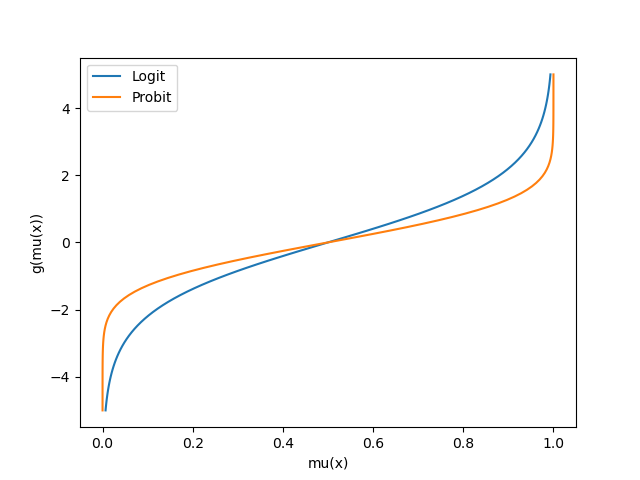
\includegraphics[scale=0.5]{img/probit_logit.png}
            \caption{Logit and Probit Functions}
            \label{fig:logit_probit}
        \end{figure}
    \end{enumerate}
    \end{example}

    Now there are many choices of functions we can take. In fact, if $\mu$ lives in $(0, 1)$, then we can really just take our favorite distribution that has a density that is supported everywhere in $\mathbb{R}$ and take the inverse cdf as our link. So far, we have no reason to prefer one function to another, but in the next section, we will see that there are more natural choices. 

    \subsubsection{Canonical Link Functions}

      Now let's summarize what we have. We assume that the conditional distribution $Y \mid X = x$ follows a distribution in the exponential family, which we can completely characterize by the cumulant generating function $\psi$. For different values of $x$, the conditional distribution will be paramaterized by different $\eta (x)$, and the resulting distribution $P_\eta$ will have some mean $\mu(x)$, which is usually not the natural parameter $\eta$. Now, let's forget about our knowledge that $\psi^\prime(\eta) = \mu$, but we know that there is some relationship between $\eta \leftrightarrow \mu$.

      Given an $x$, I need to use the linear predictor $x^T \beta$ to predict $\mu(x)$, which can be done through the link function $g$. 
      \[g\big( \mu(x) \big) = x^T \beta\]
      Now what would be a natural way of choosing this $g$? Note that our natural parameter $\eta$ for this canonical family takes value on the entire real line. I must construct a function $g$ that maps $\mu$ onto the entire real line, and so why not make it map to $\eta$. Therefore, we have 
      \[\eta(x) = g\big( \mu(x) \big) = x^T \beta\]

      \begin{definition}[Canonical Link]
      The function $g$ that links the mean $\mu$ to the canonical parameter $\theta$ is called the \textbf{canonical link}. 
      \[g(\mu) = \theta\]
      Now using our knowledge that $\psi^\prime(\eta) = \mu$, we can see that 
      \[g = (\psi^\prime)^{-1}\]
      This is indeed a valid link function. 
      \begin{enumerate}
          \item $\psi^{\prime\prime} > 0$ since it models the variance, and so $\psi^\prime$ is strictly increasing and so $g = (\psi^\prime)^{-1}$ is also strictly increasing. 
          \item The domain of $\psi^\prime$ is the real line since it takes in the natural parameter $\eta$ which exists over $\mathbb{R}$, so $\mathrm{Im}(g) = \mathbb{R}$. 
      \end{enumerate}
      \end{definition}

      So, given our cumulant generating function $\psi$ and our link function $g$, both satisfying 
      \[\psi^\prime (\eta) = \mu \text{ and } g(\mu) = x^T \beta\]
      we can combine them to get 
      \[(g \circ \psi^\prime) (\eta) = g(\mu) = x^T \beta\]
      and so, even though the mean of the response variable is not linear with respect to $x$, the value of $(g \circ \psi^\prime) (\eta)$ is indeed linear. In fact, if we choose the canonical link, then the equation 
      \[\eta = x^T \beta\]
      means that the natural parameter of our conditional distribution in the exponential family is linear with respect to $x$! From this we can find the conditional mean $\mu(x)$. 

      The reason we focus on canonical link functions is because, when the canonical link is used, the components of the model (the parameters of the linear predictor) have an additive effect on the response variable in the transformed (linked) scale, which makes the interpretation of the results easier. It's also worth noting that while using the canonical link function has some desirable properties, it is not always the best or only choice, and other link functions may be used if they provide a better fit for the data or make more sense in the context of the problem at hand.

      Let us evaluate some canonical link functions. 

      \begin{example}
      The Bernoulli has the canonical exponential form of 
      \[p_\eta (x) = \exp \big[ x \eta - \log (1 + e^\eta) \big]\]
      where $\eta = \log \big( \frac{\theta}{1 - \theta} \big)$. Since we have prior knowledge that $\theta = \mu$ (i.e. the expectation of a Bernoulli is the hyperparameter $\theta$ itself), we have a function that maps $\mu \mapsto \eta$. 
      \[\eta = g(\mu) = \log \bigg( \frac{\mu}{1 - \mu} \bigg)\]
      which gives us our result. We can also take the inverse of $\psi^\prime = \frac{e^\eta}{1 + e^\eta}$ to get our result 
      \[g (\mu) = (\psi^\prime)^{-1} (\mu) = \log \bigg( \frac{\mu}{1 - \mu} \bigg) \]
      \end{example}

  \subsection{Likelihood Optimization}

    Now let us have a bunch of data points $\{(x_n, y_n)\}_{n=1}^N$. By our model assumption, we know that the conditional distribution $Y \mid X = x_n$ is now of an exponential family with parameter $\eta_n = \eta (x_n)$ and density 
    \[p_{\eta_n} (y_n) = \exp \big[ y_n \eta_n - \psi(\eta_n) \big] h(y_n)\]
    Now we want to do likelihood optimization on $\beta$ (not $\eta$ or $\mu$), and to do this, we must rewrite the density function in a way so that it depends on $\beta$. Given a link function $g$, note the following relationship between $\beta$ and $\eta$: 
    \begin{align*}
        \eta_n = \eta (x_n) & = (\psi^\prime)^{-1} (\mu (x_n)) \\
        & = (\psi^{\prime})^{-1} \big( g^{-1} (x_n^T \beta )\big) \\
        & = h(x_n^T \beta) 
    \end{align*}
    where for shorthand notation, we define $h \coloneqq (g \circ \psi^\prime)^{-1}$. Subtituting this into the above likelihood, taking the product of all $N$ samples, and logarithming the equation gives us the following log likelihood to optimize over $\beta$. 
    \[\ell(\beta) = \log \prod_{n=1}^N p_{\eta_n} (y_n) = \sum_{n=1}^N y_n h(x_n^T \beta)  - \psi(h(x_n^T \beta) )\]
    where we dropped the $h(y_n)$ term at the end since it is a constant and does not matter. If $g$ was the canonical link, then $h$ is the identity, and we should have a linear relationship between $\eta (x_n) = x_n^T \beta$. This means that the $\eta_n$ reduces only to $x_n^T \beta$, which is much more simple to optimize. 
    \[\ell(\beta) = \log \prod_{n=1}^N p_{\eta_n} (y_n) = \sum_{n=1}^N y_n x_n^T \beta - \psi(x_n^T \beta)\]
    Note that the first term is linear w.r.t $\beta$, and $\psi$ is convex, so the entire sum must be concave w.r.t. $\beta$. With this, we can bring in some tools of convex optimization to solve. 



\section{Regression Analysis}

    Now we will talk about regression analysis from a statistical point of view. Regression can be used to approximate the relationship between two random variables (through a smooth function) and can be used for casual inference. Essentially, linear regression attempts to model the conditional distribution $Y \mid X$. 

  \subsection{Ordinary Least Squares}

    If we use a squared loss function, this is called \textbf{ordinary least squares}. It is a well known fact that the true regressor that minimizes this loss is 
    \begin{equation}
      f^\ast (x) = \mathbb{E}[Y \mid X = x]
    \end{equation}
    which is the conditional expectation of $Y$ given $X$. This is the true regressor function, which is the best approximation of $Y$ over the $\sigma$-algebra generated by $X$. This may or may not be linear. 

    \begin{theorem}[Least Squares Solution For Linear Regression]
      Given the design matrix $\mathbf{X}$, we can present the linear model in vectorized form: 
      \begin{equation}
        \mathbf{Y} = \mathbf{X} \boldsymbol{\beta} + \boldsymbol{\epsilon}, \; \boldsymbol{\epsilon} \sim N(\mathbf{0}, \sigma^2 \mathbf{I})
      \end{equation}
      The solution that minimizes the squared loss is 
      \begin{align*}
        \boldsymbol{\beta} & = (\mathbf{X}^T \mathbf{X})^{-1} \mathbf{X}^T \mathbf{Y} \in \mathbb{R}^d \\
        \Var(\hat{\boldsymbol{\beta}}) & = \hat{\sigma}^2 (\mathbf{X}^T \mathbf{X})^{-1} \in \mathbb{R}^{d \times d}
      \end{align*}
    \end{theorem}
    \begin{proof}
      The errors can be written as $\boldsymbol{\epsilon} = \mathbf{Y} - \mathbf{X} \boldsymbol{\beta}$, and you have the following total sum of squared errors: 

      \[S(\boldsymbol{\beta}) = \boldsymbol{\epsilon}^T \boldsymbol{\epsilon} = (\mathbf{Y} - \mathbf{X} \boldsymbol{\beta})^T (\mathbf{Y} - \mathbf{X} \boldsymbol{\beta})\]

      We want to find the value of $\boldsymbol{\beta}$ that minimizes the sum of squared errors. In order to do this, remember the following matrix derivative rules when differentiating with respect to vector $\mathbf{x}$. 
      \begin{enumerate}
        \item $\mathbf{x}^T \mathbf{A} \mapsto \mathbf{A}$
        \item $\mathbf{x}^T \mathbf{A} \mathbf{x} \mapsto 2 \mathbf{A} \mathbf{x}$
      \end{enumerate}
      Now this should be easy. 
      \begin{align*}
          S(\boldsymbol{\beta}) & = \mathbf{Y}^T \mathbf{Y} - \boldsymbol{\beta}^T \mathbf{X}^T \mathbf{Y} - \mathbf{Y}^T \mathbf{X} \boldsymbol{\beta} + \boldsymbol{\beta}^T \mathbf{X}^T \mathbf{X} \boldsymbol{\beta} \\
          & = \mathbf{Y}^T \mathbf{Y} - 2 \mathbf{Y}^T \mathbf{X} \boldsymbol{\beta} + \boldsymbol{\beta}^T \mathbf{X}^T \mathbf{X} \boldsymbol{\beta} \\
          \frac{\partial}{\partial \boldsymbol{\beta}} S(\boldsymbol{\beta}) & = - 2 \mathbf{X}^T \mathbf{Y} + 2 \mathbf{X}^T \mathbf{X} \boldsymbol{\beta}
      \end{align*}
      and setting it to $\mathbf{0}$ gives 
      \[2 \mathbf{X}^T \mathbf{X} \boldsymbol{\beta} - 2 \mathbf{X}^T \mathbf{Y} = 0 \implies \mathbf{X}^T \mathbf{X} \boldsymbol{\beta} = \mathbf{X}^T \mathbf{Y}\]
      and the variance of $\boldsymbol{\beta}$, by using the fact that $\Var[\mathbf{A} \mathbf{X}] = \mathbf{A} \Var[X] \mathbf{A}^T$, is
      \[\Var(\hat{\boldsymbol{\beta}}) =
       (\mathbf{X}^{\prime} \mathbf{X})^{-1} \mathbf{X}^{\prime}
       \;\sigma^2 \mathbf{I} \; \mathbf{X}  (\mathbf{X}^{\prime} \mathbf{X})^{-1}
      = \sigma^2 (\mathbf{X}^{\prime} \mathbf{X})^{-1} (\mathbf{X}^{\prime}
       \mathbf{X})  (\mathbf{X}^{\prime} \mathbf{X})^{-1}
      = \sigma^2  (\mathbf{X}^{\prime} \mathbf{X})^{-1}\]
      But we don't know the true $\sigma^2$, so we estimate it with $\hat{\sigma}^2$ by taking the variance of the residuals. Therefore, we have 
      \begin{align*}
          \boldsymbol{\beta} & = (\mathbf{X}^T \mathbf{X})^{-1} \mathbf{X}^T \mathbf{Y} \in \mathbb{R}^d \\
          \Var(\hat{\boldsymbol{\beta}}) & = \hat{\sigma}^2 (\mathbf{X}^T \mathbf{X})^{-1} \in \mathbb{R}^{d \times d}
      \end{align*}
    \end{proof}

    Note that we have assumed that $\mathbf{X}^T \mathbf{X}$ was invertible in order for such a solution to be unique, i.e. $\mathbf{X}$ must be full rank. This process breaks down when it isn't invertible, e.g. if there are repetitions in the features (one feature is a linear combination of the others and hence not full column rank). We will talk more about this soon. 

    \begin{definition}[Hat Matrix]
      For convenience of notation, let's call 
      \begin{equation}
        \mathbf{H} = \mathbf{X} (\mathbf{X}^T \mathbf{X})^{-1} \mathbf{X}^T 
      \end{equation}
      the $n \times n$ \textbf{hat matrix}, which is essentially a projection of the observed $y_i$'s to the predictions. 
      \begin{equation}
        \hat{\mathbf{y}} = \mathbf{H} \mathbf{y}
      \end{equation}
    \end{definition}

    \begin{lemma}[Properties]
      The hat matrix is an orthogonal projection matrix that projects to the column space of $\mathbf{X}$. 
    \end{lemma}

    Note that this parallels the orthogonal projection of conditional expectation to the true function onto the subspace of $X$ measurable functions. Except that we are not doing this in function space, but rather the sample space $\mathbb{R}^n$. 

    We can also see that the residuals $\hat{\epsilon}_i = y_i - \hat{y}_i$ has the property that 
    \begin{equation}
      \hat{\boldsymbol{\epsilon}} = \mathbf{y} - \hat{\mathbf{y}} = (\mathbf{I}_n - \mathbf{H}) \mathbf{y} 
    \end{equation}

    Now if we look back to the derivative of the loss $S$, we really want to set 
    \begin{equation}
      \mathbf{X}^T (\mathbf{y} - \mathbf{X} \hat{\boldsymbol{\beta}}) = \mathbf{X}^T \hat{\boldsymbol{\epsilon}} = \mathbf{0}
    \end{equation}

  \subsection{Gauss-Markov Theorem}

    At this point, we have only talked about the mathematical properties of the least squares regression, but now let's talk about some statistical properties. In machine learning, we talk about some assumptions (homoscedacity, uncorrelated residuals, etc.), and we now formalize their need. 

    \begin{theorem}[Gauss-Markov Theorem]
      Given a dataset with 
      \begin{enumerate}
        \item mean zero residuals $\mathbb{E}[\epsilon_i] = 0$, i.e. $\mathbb{E}[\mathbf{Y} \mid \mathbf{X}] = \mathbf{X} \boldsymbol{\beta}$. 
        \item homoscedacity $\mathrm{Var}[\epsilon_i] = \sigma^2 < \infty$ for all $i$, 
        \item uncorrelated residuals $\mathrm{Cov}(\epsilon_i, \epsilon_j) = 0$ for all $i \neq j$. This and the previous assumption can be combined into $\mathrm{Cov}[\mathbf{Y} \mid \mathbf{X}] = \sigma^2 \mathbf{I}_n$. 
      \end{enumerate}
      We were concerned with estimating the parameters $\beta_1, \ldots, \beta_d$. Now let's generalize this and consider the problem of estimating, for some known constants $c_1, \ldots, c_{d+1}$, the point estimator 
      \begin{equation}
        \theta = c_1 \beta_1 + c_2 \beta_2 + \ldots + c_d \beta_d + c_{d+1}
      \end{equation}
      Then the estimator 
      \begin{equation}
        \hat{\theta} = c_1 \hat{\beta}_1 + c_2 \hat{\beta}_2 + \ldots + c_d \hat{\beta}_d + c_{d+1}
      \end{equation}
      where $\hat{\beta_i}$ is clearly an unbiased estimator of $\theta$ and it is a linear estimator of $\theta$, i.e. 
      \begin{equation}
        \hat{\theta} = \sum_{i=1}^n b_i y_i
      \end{equation}
      for some known (given $\mathbf{X}$) constants $b_i$. Then, the Gauss-Markov theorem states that the estimator $\hat{\theta}$ has the smallest (best) variance among \textit{all} linear unbiased estimators of $\theta$, i.e. $\hat{\theta}$ is BLUE. 
    \end{theorem}

  \subsection{Analysis of variance (ANOVA)}


\bibliography{./bibfile}
\bibliographystyle{alpha}
\end{document}
